\documentclass[usenatbib,fleqn]{mnras}

\makeatletter
\newlength{\abovecaptionskip}%
\setlength{\abovecaptionskip}{10\p@}
\makeatother


\usepackage{threeparttable}
 

\usepackage{amsmath,amssymb}
\usepackage{cases}
\usepackage{mathrsfs}
\usepackage{graphicx}
\usepackage{epstopdf}
%\usepackage{hyperref}
\epstopdfsetup{outdir=./figures/}
\graphicspath{{./figures/}}
\usepackage{url}
%\usepackage{aas_macros}

\newcommand\lsim{\mathrel{\rlap{\lower4pt\hbox{\hskip1pt$\sim$}}
    \raise1pt\hbox{$<$}}}
\newcommand\gsim{\mathrel{\rlap{\lower4pt\hbox{\hskip1pt$\sim$}}
    \raise1pt\hbox{$>$}}}


\newcommand       \be          {\begin{eqnarray}}
\newcommand       \ee          {\end{eqnarray}}
\newcommand{\Mbh}[1][]{M_{\bullet1}}
\newcommand{\Menc}{M_{\rm enc}}
\renewcommand{\th}{t_h}
\newcommand{\Msun}{{\rm M_\odot}}
\newcommand{\pyear}{{\rm yr}^{-1}}
\newcommand{\rs}{r_s}

% write title (with email and institute)
\title[Influence of CNM on TDE radio emission]{The influence of the
  cicumnuclear environment on the radio emission from TDE jets}
\author[Generozov et al.]{ A. Generozov$^{1}$, P. Mimica$^{2}$,
  B. D. Metzger$^{1}$, D. Giannios$^{3}$, N. Stone$^{1}$,
  M.A. Aloy$^{2}$
  \\
  $^{1}$Columbia Astrophysics Laboratory, Columbia University, 550 West 120th Street, New York, NY 10027\\
  $^{2}$Departamento de Astronomia y Astrofisica, Universidad de Valencia, E-46100 Burjassot, Spain\\
  $^{3}$Department of Physics and Astronomy, Purdue University, 525
  Northwestern Avenue, West Lafayette, IN 47907, USA}

\begin{document}
\maketitle
\begin{abstract}
  There are now dozens of candidates for tidal disruptions of stars by
  supermassive black holes (TDEs) at optical and x-ray wavelengths. A
  small fraction of these events, (e.g. {\it Swift} J1644+57) have radio
  synchrotron emission consistent with a powerful, relativistic jet
  shocking surrounding gas. The low detection rate of such events may
  mean that powerful jets are intrinsically rare in TDEs. However, it
  could also mean that typical nuclear gas densities are unfavorable
  for producing observable radio emission. We explore this
  possibility, constraining the range of gas densities which could be
  encountered by a TDE jet. We then calculate radio light curves for
  jets across the expected range of gas densities ($\sim$ 0.5-2000
  cm$^{-3}$ at $10^{18}$ cm). We find bright radio transients across
  this range of density profiles. Existing radio upper limits are
  often taken decades after the observed flare, well after the
  expected peak of the light curve for low density
  environments. Nonetheless they exclude powerful, {\it Swift} J1644+57-like
  jets for CNM densities less than 60 cm$^{-3}$ at $10^{18}$ cm. More
  stringent constraints would be possible with prompt follow-up of
  tidal disruption event candidates and would inform our understanding
  of the conditions necessary to launch jets.
\end{abstract}
\section{Introduction}
\label{sec:intro}
When a star in a galactic nucleus is deflected too close to the
central supermassive black hole (BH), it can be torn apart by tidal
forces.  During this tidal disruption event (TDE), roughly half of the
stellar debris remains bound to the BH, while the other half is flung
outwards and unbound from the system.  The bound material, following a
potentially complex process of debris circularization
(\citealt{Guillochon+2013},\citealt{Hayasaki+2013},\citealt{Hayasaki+2015},\citealt{Shiokawa+2015},\citealt{Bonnerot+2015}),
accretes onto the BH, creating a luminous flare lasting months to
years \citep{Hills1975, Carter+1982, Rees1988}.

Many TDE flares have now been identified at optical/ultraviolet (UV)
\citep{Gezari+2008, Gezari+2009, van-Velzen+2011, Gezari+2012,
  Arcavi+2014, Chornock+2014, Holoien+2014, Vinko+2015, Holoien+2016}
and soft x-ray wavelengths \citep{Bade+1996, Grupe+1999,
  Komossa&Greiner1999, Greiner+2000, Esquej+2007, Maksym+2010,
  Saxton+2012}. Beginning with the discovery of {\it Swift} J1644+57
(hereafter SwJ1644) in 2011, three additional TDEs have been
discovered by their hard x-ray emission (\citealt{Bloom+2011,
  Levan+2011, Burrows+2011, Zauderer+2011, Cenko+2012, Pasham+2015,
  Brown+2015}).  Unlike the optical/UV and soft X-ray TDEs, these
events are the result of non-thermal emission from a transient
relativistic jet beamed along our line of sight, similar to the blazar
geometry of active galactic nuclei (AGN).  In addition to their highly
variable X-ray emission, which likely originates from the base of the
jet, these events are characterized by radio synchrotron emission.
The latter, more slowly evolving, is powered by shocks formed at the
interface between the jet and surrounding circumnuclear medium (CNM)
\citep{Bloom+2011,Giannios&Metzger2011,Metzger+2012,De-Colle+2012,Mimica+2015},
analagous to the afterglow of a gamma-ray burst.

Although a handful of jetted TDE flares have been observed, their
volumetric rate is a very small fraction $\sim 10^{-5}-10^{-4}$ of the
observed TDE flare rate (e.g., \citealt{Burrows+2011},
\citealt{Brown+2015}), and an even smaller fraction of the
theoretically predicted TDE rate
\citep{Wang&Merritt2004,Stone&Metzger2016}.  One potential explanation
for this discrepancy is that the majority of TDEs produce powerful
jets, but their hard X-ray emission is relativistically beamed into a
small angle $\theta_{\rm b}$, making them visible to only a small
fraction of observers.  However, the inferred beaming fraction $f_b
\approx \theta_{b}^{2}/2 \sim 10^{-5}-10^{-4}$ would require
$\theta_{\rm b} \sim 0.01$ and hence a jet with a bulk Lorentz factor
of $\Gamma \gtrsim 1/\theta_j \sim 100$, much higher than typically
inferred for AGN jets or inferred for SwJ1644
(\citealt{Metzger+2012}).

The low detection rate of hard X-ray TDEs may instead indicate that
jets are intrinsically rare in these events, or that the conditions of the
surrounding environment are unfavorable for producing bright emission.
Jets could be rare if they require, for instance, a highly
super-Eddington accretion rate (\citealt{De-Colle+2012}), a TDE from a
deeply plunging stellar orbit (\citealt{Metzger&Stone2015}), or a
particularly strong magnetic flux threading the star
(\citealt{Tchekhovskoy+2014,Kelley+2014}).  Alternatively, jet formation
or its X-ray emission could be suppressed if the disk undergoes
Lens-Thirring precession due to a misalignment between the angular
momentum of the BH and that of the disrupted star
(\citealt{Stone&Loeb2012}).  In the latter case, however, even a `dirty'
jet could still be produced, which emits luminous non-thermal radio
synchrotron emission as it interacts the surrounding CNM.  The radio
emission from an off-axis is predicted to be relatively isotropic
\citep{Giannios&Metzger2011,Mimica+2015}.

\citet{Bower+2013} and \citet{van-Velzen+2013} performed follow-up
radio observations of optical/UV and soft X-ray TDE flares timescales
of months to decades after the outburst (see Table 1 of
\citealt{Mimica+2015} for a compilation). They find no radio afterglows
definitively associated with the host galaxies of strong TDE
candidates.\footnote{There were radio detections for two ROSAT flares:
  RX J1420.4+5334 and IC 3599. However, for RX J1420.4+5334 the radio
  emission was observed in a different galaxy than was originally
  associated with the flare.  IC 3599 has shown multiple outbursts in
  the recent years, calling into question whether it is a true TDE at all
  \citep{Campana+2015}.}  \citet{Bower+2013} and
\citet{van-Velzen+2013} use a simple model for the radio emission as a
Sedov blast wave, to conclude that $\lesssim 10\%$ of TDEs produce
jetted TDE emission at a level similar to that produced in SwJ1644.  \citet{Mimica+2015} used 2D hydrodynamical models, coupled
with a synchrotron radiation transport calculation, to model the
on-axis emission from SwJ1644. They then extended this
model to off-axis viewing angles, and concluded that most previous
TDEs should have been detected if their jets were as powerful. 

Recently, a candidate TDE flare (ASSASN-14li) was observed to
have transient radio emission, consistent with either a weak
relativistic jet \citep{van-Velzen+2015} or a sub-relativistic outflow
\citep{Alexander+2015} with a total energy of
$\sim 10^{48}-10^{49}$ ergs.  ASSASN-14li occurred in a very nearby galaxy,
and if other TDE candidates launched similar outflows, their radio
afterglows would be below existing upper limits. A priori it
is not obvious whether the lack of observed radio emission in most
thermal TDEs is due to (i) weak/no outflows or (ii) a nuclear gas
environment unfavorable for producing observable radio emission.

Previous works (\citealt{Bower+2013}; \citealt{van-Velzen+2013};
\citealt{Mimica+2015}) have generally assumed that all TDEs occur in a
similar environment as SwJ1644.  However, in general the
gas density in a galactic nucleus depends sensitively on the sources
of gas from stellar winds, and the sources of gas heating
(\citealt{Quataert2004,Generozov+2015}).  In a normal gamma-ray burst, the
environment the jet emerges from is relatively well-understood to be
the wind of the massive progenitor star, or the ISM of the host
galaxy.  However, the density of the CNM encountered by a TDE jet
could in principle be orders of magnitude higher.

In this paper we address the range of gas densities encountered by
jetted TDEs and estimate their synchrotron emission by means of
analytic calculations and numerical simulations.  We find that radio
emission should be detected for all plausible CNM densities, leading
to the robust conclusion that most TDEs do not launch SwJ1644-like
jets.  This result has significant implications for the physics of jet
launching in TDEs and other accretion flows.

In $\S\ref{sec:cnm}$ we use the formalism developed in
\citet{Generozov+2015} (hereafter GSM15) to calculate the CNM profiles
encountered by TDE jets for different assumptions about the stellar
population in the galactic nucleus.  A younger stellar population
produces significant wind mass loss from O and B stars. In contrast,
the rate of wind mass loss from an older population, which lacks these
massive stars, could be a $\sim$couple orders of magnitude smaller.
We show that the requirement of a physical stellar population limits
the gas density on a scale of $10^{18}$ cm to a range of $n_{18} \sim
0.5-2000$ cm$^{-3}$. We also show that the measured distribution of
accretion rates of low mass SMBHs in the local universe suggests that
the gas density in most galactic nuclei lie within a similar range.

As a second component of this paper, in $\S\ref{sec:results}$ we
explore the expected synchrotron emission for different energy jets
across the allowed range of CNM conditions. 
%  Then in
% $\S\ref{sec:numerical}$ use both 1D and 2D hydrodynamic models to
% simulate the jet propagating through the CNM and compare the results
% in $\S\ref{sec:2D}$. In $\S\ref{sec:results}$ we show radio light
% curves from our 1D models for a wide range of CNM densities, to
% illustrate qualitatively how much varying the CNM density by itself
% could change the radio light curve. 
We present analytic scaling relations for the time of peak and peak
flux of the radio light curve in Appendix~\ref{app:analyt}. We
summarize our conclusions in $\S\ref{sec:conc}$.

\section{Range of CNM Densities}
\label{sec:cnm}

In this section we place constraints on the gas densities in galactic nuclei.  In $\S\ref{sec:analy}$, we determine the
possible range of densities resulting from mass loss by stellar
winds. Then in $\S\ref{sec:empirical}$ we convert empirical
distributions for black hole luminosities into distributions of
nuclear gas densities.  

\subsection{Analytic Constraints on CNM Density}
\label{sec:analy}

\subsubsection{Preliminary Considerations}

The radio emission of a jet is primarily sensitive to the density of
ambient gas near the Sedov radius, outside of which the jet has
swept up a gaseous mass exceeding its own. For a power law gas density
profile, $n= n_{18} \left(r/r_{18}\right)^{-k}$,
\begin{equation}
  r_{\rm sed} = r_{18} \left( \frac{E(3-k)}{4\pi n_{0}
      m_{\rm p} c^2 r_{18}^3} \right)^{1/(3-k)} \approx 3 E_{54}^{1/2} n_{\rm 18}^{-1/2}\,{\rm pc}. 
  \label{eq:rdec}
\end{equation}
where $E = E_{54}10^{54}$ erg is the isotropic equivalent energy,
$r_{18} = r/10^{18}$ cm, and in the final equality we have taken $k =
1$.  For a powerful jet similar to SwJ1644, the deceleration radius is
typically of order a parsec.

An initially relativistic jet will slow to sub-relativistic speeds at
$r \sim r_{\rm sed}$.  However, deceleration sets in earlier, once the
jet has swept up a fraction $\sim 1/\Gamma$ of its rest mass, as
occurs at the radius
\begin{equation}
  r_{\rm dec}=\frac{r_{\rm sed}}{\Gamma^{2/(3-k)}}.
  \label{eq:rdec2}
\end{equation}
%
The jet reaches
 the Sedov and deceleration radii, respectively, at
observer times 
\begin{equation}
t_{\rm sed} = \frac{c}{r_{\rm sed}} \approx
10 E_{54}^{-1/2}n_{18}^{1/2} {\rm year}
 \end{equation} 

\begin{equation}
t_{\rm dec} =
\frac{c}{2\Gamma^{2} r_{\rm dec}} = \frac{t_{\rm
    sed}}{2\Gamma^{3(4-k)/(3-k)}} = \frac{t_{\rm sed}}{2\Gamma^{3}},
 \label{eq:tdec}
\end{equation}
%
where in the final equality we have again taken $k = 1$.


\subsubsection{Dynamical Model of CNM}
\label{sec:model}

The dominant source of gas in the CNM of quiescent galaxies is winds
from stars in the galactic nucleus. We model the hot phase of the ISM
using the 1D spherical hydrodynamic equation with mass and energy
injection from stellar winds (e.g. \citealt{Holzer+1970};
\citealt{Quataert2004})
\begin{align}
  &\frac{\partial \rho}{\partial t}+\frac{1}{r^2}\frac{\partial}{\partial r}\left(\rho r^2 v\right)=q \label{eq:drhodt}\\
  &\rho \left(\frac{\partial v}{\partial t} + v\frac{\partial
      v}{\partial r}\right) =-\frac{\partial p}{\partial r}- \rho\frac{GM_{\rm enc}}{r^{2}} -q v \label{eq:dvdt}\\
  &\rho T\left(\frac{\partial s}{\partial t} + v\frac{\partial
      s}{\partial
      r}\right)=q\left[\frac{v^2}{2}+\frac{v_w^2}{2}-\frac{\gamma}{\gamma-1}
    \frac{p}{\rho} \right] ,
\label{eq:model}
\end{align}
where $\rho = \mu m_p n$, $v$, $p$, and $s$ are the density, velocity,
pressure (assumed to be an ideal gas with $\mu = 0.62$), and specific
entropy, respectively.  The enclosed mass $\Menc = M_{\bullet} +
M_{\star}$ includes both the black hole mass $M_{\bullet}$ and
enclosed stellar mass $M_{\star} \propto \int \rho_{\star}r^{2}dr$,
where $\rho_{\star}$ is the stellar density. At the radius of the
sphere of influence, $r_{\rm inf}$, the enclosed stellar and black
masses are equal, $M_{\star}(r_{\rm inf})=\Mbh$.  We take $r_{\rm
  inf}=3.5 \Mbh[,7]^{0.6}$ (GSM15), where $\Mbh[,7]=\Mbh/10^7 \Msun$.

The mass source term $q =\eta \rho_\star/\th$ is the mass injection
rate per unit volume per unit time. The energy source term $\propto
v_w^{2}$, parameterizes the heating rate of the gas, as physically
results from stellar wind kinetic energy, supernovae, and black hole
feedback.

GSM15 present analytic approximations for the
densities and temperatures of steady state solutions to
equation~\eqref{eq:model}. We apply these results across the
physically allowed range heating rates ($v_w$) and mass injection
rates ($\eta$), and obtain the corresponding range of gas densities.

\subsubsection{Stellar density profiles}
We assume a broken power law for the stellar density profile,
$\rho_{\star}$, motivated by Hubble measurements of the radial surface
brightness profiles for hundreds of nearby early type galaxies
\citep{Lauer+2007}.  The measured profile is well fit by the so-called
``Nuker'' law parameterization, i.e.~a piece-wise power law that smoothly
transitions from an inner power law slope, $\Gamma$, to an outer power
law slope, $\beta$, at a break radius, $r_b$.

Most galaxies have $0<\Gamma<1$, and are classified into two broad
categories: ``core" galaxies with $\Gamma<0.3$ and ``cusp" galaxies with
$\Gamma>0.5$. Assuming spherical symmetry and a constant mass-to-light
ratio, the inner stellar profile translates to a stellar density of
$\rho_\star\propto r^{-1-\Gamma}=r^{-\delta}$. Core galaxies have
$1<\delta<1.3$, while cusp galaxies have $1.5<\delta<2$.

Cusp-like stellar density profiles, are the most relevant to TDEs for
two reasons.  First, only a low mass black hole ($\Mbh\lsim 10^8
\Msun$) can disrupt a main sequence star, and low mass low mass black
holes are more commonly characterized by cusp-like profiles.
Additionally, as described in \citet{Stone&Metzger2016} a cuspy
stellar density profile results in a higher TDE rate per galaxy.  We
adopt a fiducial value of $\Gamma=0.7$ ($\delta=1.7$), motivated by
the rate-weighted average value of the inner stellar density profile for
the galaxies in \citet{Stone&Metzger2016} (their Table C).


 {\bf Recently changed from $\delta=1.8$, need to
  double check all expressions.}

\subsubsection{Gas density profiles}


Given sufficiently strong heating, a one-dimensional steady-state
model for the CNM is characterized by an inflow-outflow structure.
The velocity passes through zero at the ``stagnation radius'', $\rs$.
Mass loss from stars interior to the stagnation radius is accreted,
while that outside of $\rs$ is unbound in an outflow from the nucleus.
Fig.~\ref{fig:profiles} shows example radial profiles of the
steady-state gas density calculated for a core and a cusp stellar
density profile. The stagnation radius is marked as a blue dot on each
profile.

As described in GSM15, the stagnation radius is approximately given by
\begin{equation}
r_s \simeq f(\delta) \frac{G M}{v_w^2},
\label{eq:rs}
\end{equation}
%
where $f(\delta)$ is a constant of order unity that depends on the
slope of the stellar density profile $\delta$.  The gas density at the
stagnation radius, $n(\rs)$, is determined by the rate at which
stellar winds inject mass interior to this,
\begin{equation}
  \dot{M}=\frac{\eta M_{\rm \star}(\rs)}{t_h} \approx  3.0 \times 10^{-6} \Mbh[,7]^{0.22} \eta_{0.02} \left(\frac{r_s}{\rm
      pc}\right)^{1.3} \Msun \, {\rm yr}^{-1},
\label{eq:dotM}
\end{equation}
where $M_{\star}(\rs)$ is the total stellar mass enclosed within the
stagnation radius and the second equality was derived for our fiducial
value of $\delta=1.7$, where $\eta_{0.02}=\eta/0.02$ is normalized to
a fiducial value characteristic of an old stellar population.

The density at the stagnation radius, $n(\rs)$, is estimated by
equating the gas injected by stellar winds over a dynamical time at
the stagnation radius, $t_{\rm dyn} (\rs)=(\rs^3/G \Mbh)^{1/2}$, to
the gas mass enclosed at this location.  This gives
\begin{align}
  &\frac{4 \pi}{3} \rs^3 \mu m_p n(r_s) \simeq \dot{M} t_{\rm dyn}
  (\rs) \nonumber\\
  &\Rightarrow n(r_s) \simeq 0.21 \eta_{0.02} \Mbh[,7]^{-0.28} \left(\frac{r_s}{\rm
      pc}\right)^{-0.2} {\rm cm}^{-3}.
\label{eq:nrs}
\end{align}
%
Substituting equation~\eqref{eq:rs} for $r_s$, we obtain 
\begin{equation}
n(r_s) \simeq 0.2 \, v_{500}^{0.4} \eta_{0.02} \Mbh[,7]^{-0.48} {\rm cm}^{-3},
\label{eq:nrs2}
\end{equation}
where $v_{500}=v_w/\left(500 \,\mathrm{km\,\,
    s^{-1}}\right)$. 
%
Near the stagnation radius, GSM15 found that the radial gas profile
has a power-law slope of $k \approx (4\delta-1)/6$, which for our
fiducial value of $\delta$=1.7 gives $n \propto r^{-1}$.  A similar
density profile obtains for most radii of interest.\footnote{For cusp
  galaxies, the gas velocity asymptotes to a constant value between
  the stagnation radius and break radius (provided they are
  sufficiently far apart). In this region we instead expect $n\propto
  r^{1-\delta}$.}  Thus, we adopt $n(r)= n_{18} (r/10^{18} {\rm
  cm})^{-1}$ as our fiducial density profile, where $n_{18}$ is the
density at $r = 10^{18}$ cm.  In Appendix~\ref{app:core} we explore a
core-like density profile, to which we compare our results for the
jetted radio emission to the fiducial cusp case in
$\S\ref{sec:profileComp}$.

Combining our assumed $n\propto r^{-1}$ profile with
equation~\eqref{eq:nrs}, we obtain
\begin{equation}
  n_{18}\simeq 0.6 \left(\frac{r_s}{\rm pc}\right)^{0.8}
  \Mbh[,7]^{-0.28} {\rm cm^{-3}},
  \label{eq:n18}
\end{equation}
%
Substituting the stagnation radius (eq.~\ref{eq:rs}) into this
expression gives
\begin{equation}
n_{18}\simeq 0.3 \Mbh[,7]^{0.52} \eta_{0.02} v_{500}^{-1.6} {\rm
  cm^{-3}}.
\label{eq:n182}
\end{equation} 
%
Although the gas density steepens near the break radius $r_b$ of the
stellar density profile (Fig.~\ref{fig:profiles}), this will only
affect the radio emission near its peak if $r_b$ lies inside of the
Sedov radius (eq.~\ref{eq:rdec}).  Figure \ref{fig:profiles} shows the
Sedov radius for different energy jets and the gas density profiles
there.  The measured break radii of all but four the galaxies in
\citet{Lauer+2007} exceeds 10 parsecs.  This is well outside of the
Sedov radius, even for a very energetic jet, with an isotropic
equivalent energy of $E=4\times 10^{54}$ erg in a CNM of particularly
low density, $n_{18} \sim 1$ cm$^{-3}$.

The presence of nuclear star
cluster in the galactic center could produce another break in the
stellar density profile near the outer edge of the NSC, which is
typically located at $\sim 1-5$ pc \citep{Georgiev+2014}.  However,
even a break radius of 1 pc will reside inside the Sedov radius,
except for the combination of a powerful jet and relatively small CNM
density, $n_{18}<20$ cm$^{-3}$.  Henceforth we neglect the effects of
a break in the stellar density profile in our analysis.


\begin{figure}
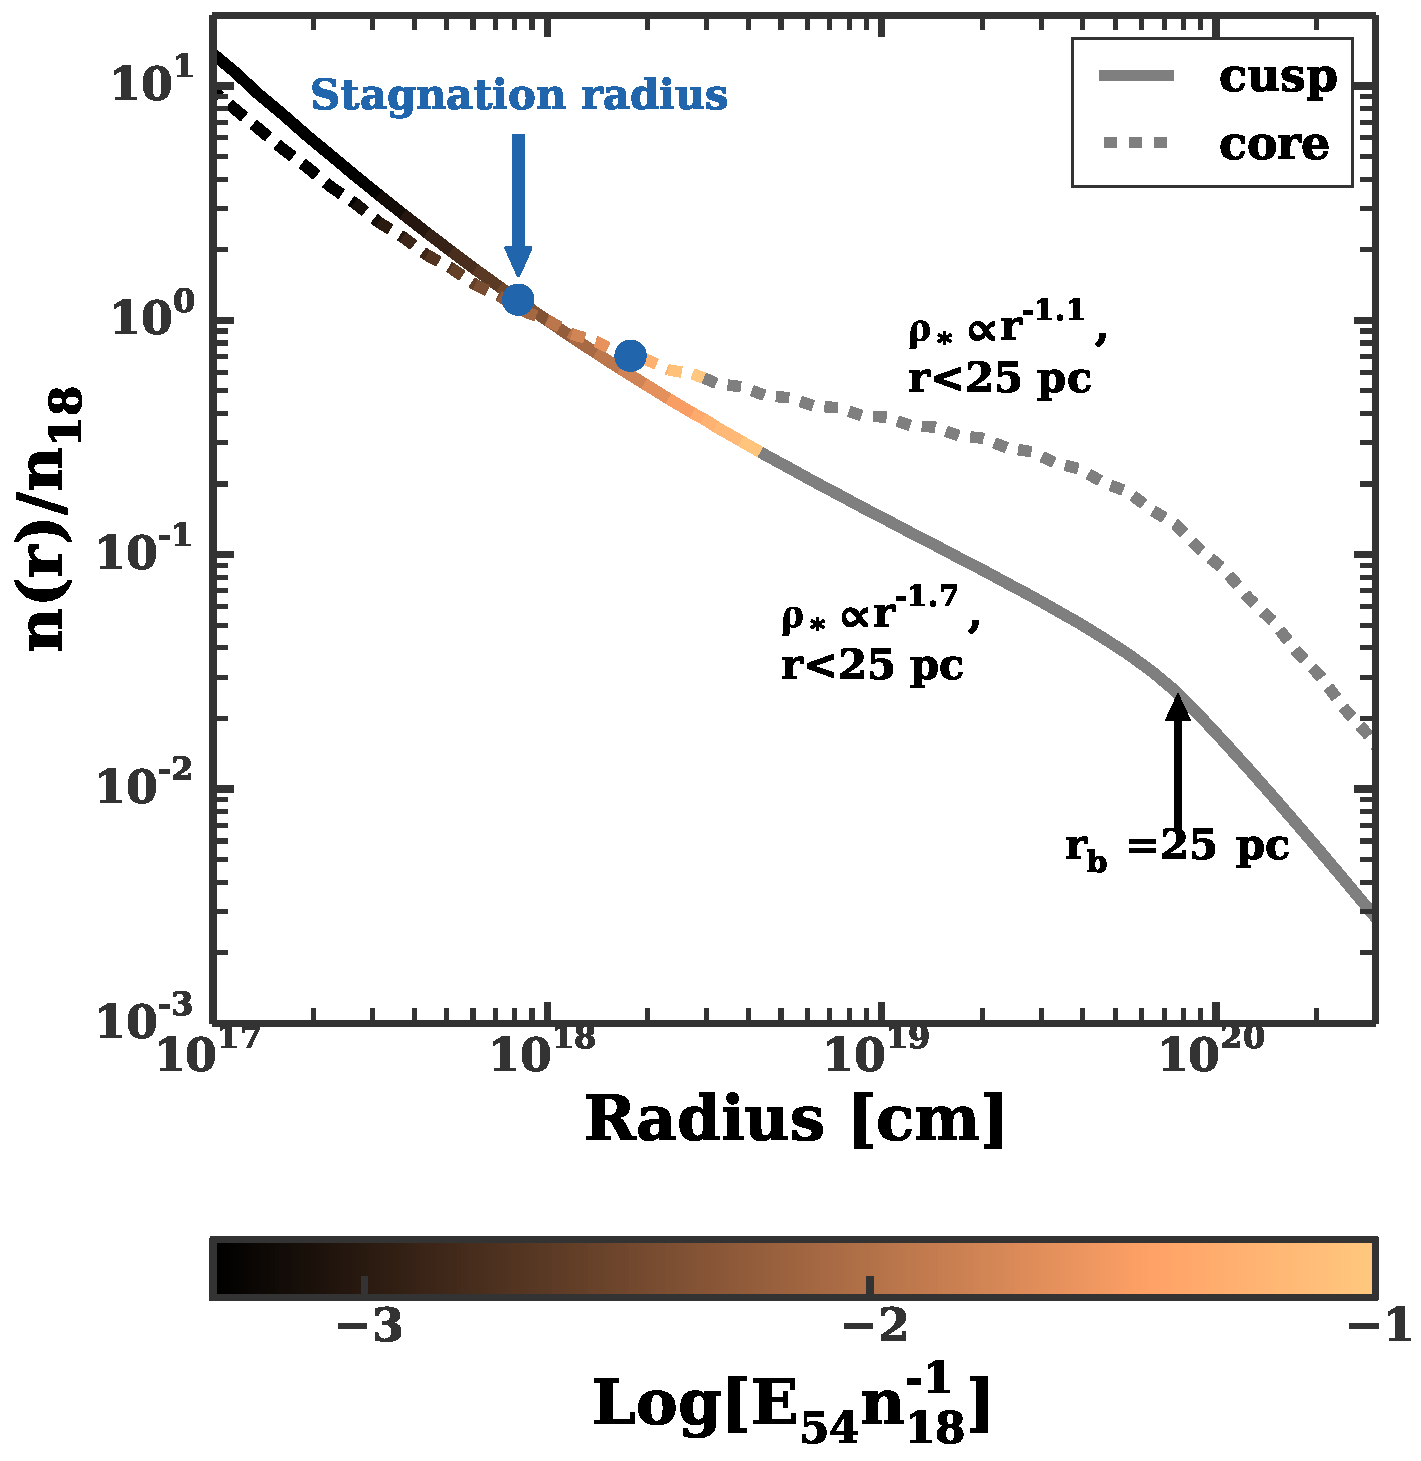
\includegraphics[width=8cm]{sedov_radius.pdf}
\caption{\label{fig:profiles} Steady-state radial profiles of the gas
  density of the CNM, $n(r)/n_{18}$, normalized to the value $n_{18} =
  n(r = 10^{18}$ cm), calculated for a black hole mass $10^{7}
  \,\Msun$ and gas heating parameter $v_w=600$ km s$^{-1}$.  Cusp and
  core stellar density profiles are shown with solid and dashed lines,
  respectively.  The line color denotes the isotropic equivalent
  energy of a jet for which the Sedov radius equals that radius from
  the black hole (given the swept up interior gaseous mass), assuming
  an initial jet Lorentz factor of $\Gamma=2$.}
\end{figure}



\subsubsection{Plausible Density Range}
\label{sec:densAllowed}

In this section, we estimate the plausible range in the normalization
of the CNM gas profile, $n_{18}$.  We assume that star formation
occurs in two bursts, an old burst of age comparable to the Hubble
time $t_{\rm h} = 10^{10}$ yr, and a ``young'' burst of variable age
$t_{\rm burst} \ll t_{\rm h}$ which contributes a fraction $f_{\rm
  burst}$.
%Both the young and old stars have the
%same (cuspy) density profile, which implies that the gas density
%profile goes as $r^{-1}$.

For a sufficiently large burst occurring less than 40 Myr ago, gas
heating is dominated by the energetic winds of massive star
winds.\footnote{Although Type II supernovae are also an important heating
  source which dominates stellar winds after $\sim$6 Myr
  \citep{Voss+2009}, they are intermittent and hence their
  contribution to the gas heating is neglected for simplicity.}  In
this case, the mass return ($\eta$) and heating parameters ($v_w$) are
calculated as described in GSM15 (their Appendix C).  Given
$\eta(t_{\rm burst},f_{\rm burst})$ and $v_w(t_{\rm burst},f_{\rm
  burst})$, we calculate $n_{18}$ following equation~\eqref{eq:n182}.

For older stellar populations, gas heating may come from a few
different sources, including Type Ia Supernovae (SNe)\footnote{Unbound
  debris streams from TDEs provide another source of heating localized
  in the galactic center (\citealt{Guillochon+2015a}), which we
  neglect.} and AGN feedback.  We focus on
quiescent phases, during which SNe Ia dominate.  As discussed in
GSM15, SNe Ia clear out the gas external to a critical radius, $r_{\rm
  Ia}$, where the interval between successive Ia SNe equals the
dynamical (gas inflow) timescale.  For an old stellar population,
$n_{18}$ is estimated by equating $r_{\rm Ia}$ with the stagnation
radius in equation~\eqref{eq:n18}.  The Ia radius is calculated as
described in GSM15 at times $t>300 \,{\rm Myr}$ after star formation,
and is taken to be constant for $t = 40-300$ Myr.\footnote{GSM15
  incorrectly extrapolated the Ia rate valid at times $t>300 \,{\rm
    Myr}$ back to a time $t = 3$ Myr, which unphysical as no white
  dwarfs would have formed by this time.  Although its qualitative
  impact on our results is minimal, here we instead take the Ia rate
  to be 0 for $ t < 40$ Myr.}

%\footnote{The Ia rate is given
 % by $8.8 \times 10^{-13} \left(\frac{t}{3\times 10^{8} {\rm
  %      yr}}\right)^{-1.12} \, \Msun^{-1} \, {\rm yr}^{-1} $ for
  %$t>3\times 10^8$ years.} =
%In GSM15 we incorrectly extrapolated this rate all of the way to 3
%Myr, which is unphysical because white dwarfs have not yet formed. Here, we instead take the Ia rate to be zero for times less than 40 Myr and constant from 40$-$300 Myr.

Fig.~\ref{fig:param} shows how $n_{18}$ varies with the young
starburst properties, $f_{\rm burst}$ and $t_{\rm burst}$.  We find a
maximum density of $n_{18} \sim 3000$ cm$^{-3}$ is achieved for a
burst of age $t_{\rm burst} \sim 4$ Myr which forms most of the stars
in the nucleus $f_{\rm burst} \sim 1$.  In this case, both the energy
and mass budgets of the CNM are dominated by fast winds from massive
stars.  Although a large gas density is present in the immediate
aftermath of a starburst, its magnitude will decline with the wind
mass loss rate, approximately $\propto t^{-3}$.  Therefore, the gas
density would decline by an order of magnitude from this maximum
allowed value after just a few Myr.

By contrast, the lowest allowed density $\sim 0.03$ cm$^{-3}$ is
achieved for a relatively modest burst of young stars $t_{\rm burst}
\approx 10^{6}$ Myr, which forms a fraction $f_{\rm burst} = 4\times
10^{-4}$ of the total stellar mass. In this case the young massive
stars provide a high heating rate, while the mass injection rate is
comparatively low and receives contributions from both young and old
stars.

Our procedure may underestimate the value of $n_{18}$ somewhat, as we
do not include the effects of discreteness on the assumed stellar
population.  In particular, we assume that massive stars provide a
spatially homogeneous heating source, even on small scales where the
number of massive stars present may be very small.  The doubly hatched
region in Fig.~\ref{fig:param} denotes the region where less than one
massive star ($\gsim 15 \Msun$) is on average present inside of the
nominal stagnation radius (eq.~\ref{eq:rs}).  Discreteness effects are
thus important for relatively small bursts of star formation,
including the case described above which gives the minimum $n_{18}$.
If we instead equate the stagnation radius to the radius enclosing a
single star of mass $\gsim 15 \Msun$, we find a larger value of
$n_{18}\sim 0.5$ cm$^{-3}$.  From this we conclude that the true
minimum density likely resides between these extremes, min($n_{18})
\sim 0.03-0.5$ cm$^{-3}$.

Most of the host galaxies of observed TDE flares show evidence of some
star formation within the last Gyr \citep{French+2016}.  In this
region of parameter space corresponding to the right side of
Fig.~\ref{fig:param}, gas heating rate is dominated by SN Ia and we
expect $n_{18}\sim 10-100$ cm$^{-3}$.
%{\bf AG note that the
 % entire stellar pop likely did not form 1 Gyr ago. In fact the
  %observation merely indicate that there was some star formation w. in
 % the last Gyr}

To summarize, we expect the CNM densities of quiescent galaxies on
parsec scales to vary from min($n_{18}) \sim 0.03$ to max($n_{18})\sim
10^{3}$ cm$^{-3}$, with a typical value of perhaps $n_{18}\sim 100$ cm$^{-3}$
in the host galaxies of observed TDEs.

\subsubsection{Mass drop-out from star formation?}

Our model for the CNM predicts the total gas density
sourced by stellar winds, including both hot and cold phases.  In the
first few Myr after a starburst, the injected stellar wind material is hot ($T\gsim 10^{7}$ K) due to the
thermalized wind kinetic energy.  Later, SNe Ia provide intermittent heating, but the stellar wind material that accumulates on small
scales, between successive SNe Ia may become much cooler, with
temperature $\lesssim 10^{4}$ K, and would condense into clumps.

The radio emission from a TDE jet is expcted to be similar for a
clumpy and a smooth medium with the same average density
(e.g.~\citealt{Nakar&Granot2007}; \citealt{Mimica&Giannios2009};
\citealt{vanEerten+2009}; $\S$~\ref{sec:empirical}).  However, cold gas
may also condense into stars.  To estimate the star formation rate, we
assume that the CNM self-regulates itself to a condition of marginal
thermal stability.  This we define as the cooling time being ten times
longer than the dynamical timescale (e.g.~\citealt{McCourt+09}). For a
$\sim$1 Gyr old stellar population, we find that this requires a star
formation rate of $5.3 \times 10^{-4} \,\Msun$ yr$^{-1}$, which
implies that only $\sim 40$\% of the gas injected on small scales
would be turned into stars.  The gas density would therfore be only a
few times lower than in our estimates which neglect mass drop out from
star formation.

\begin{figure} 
  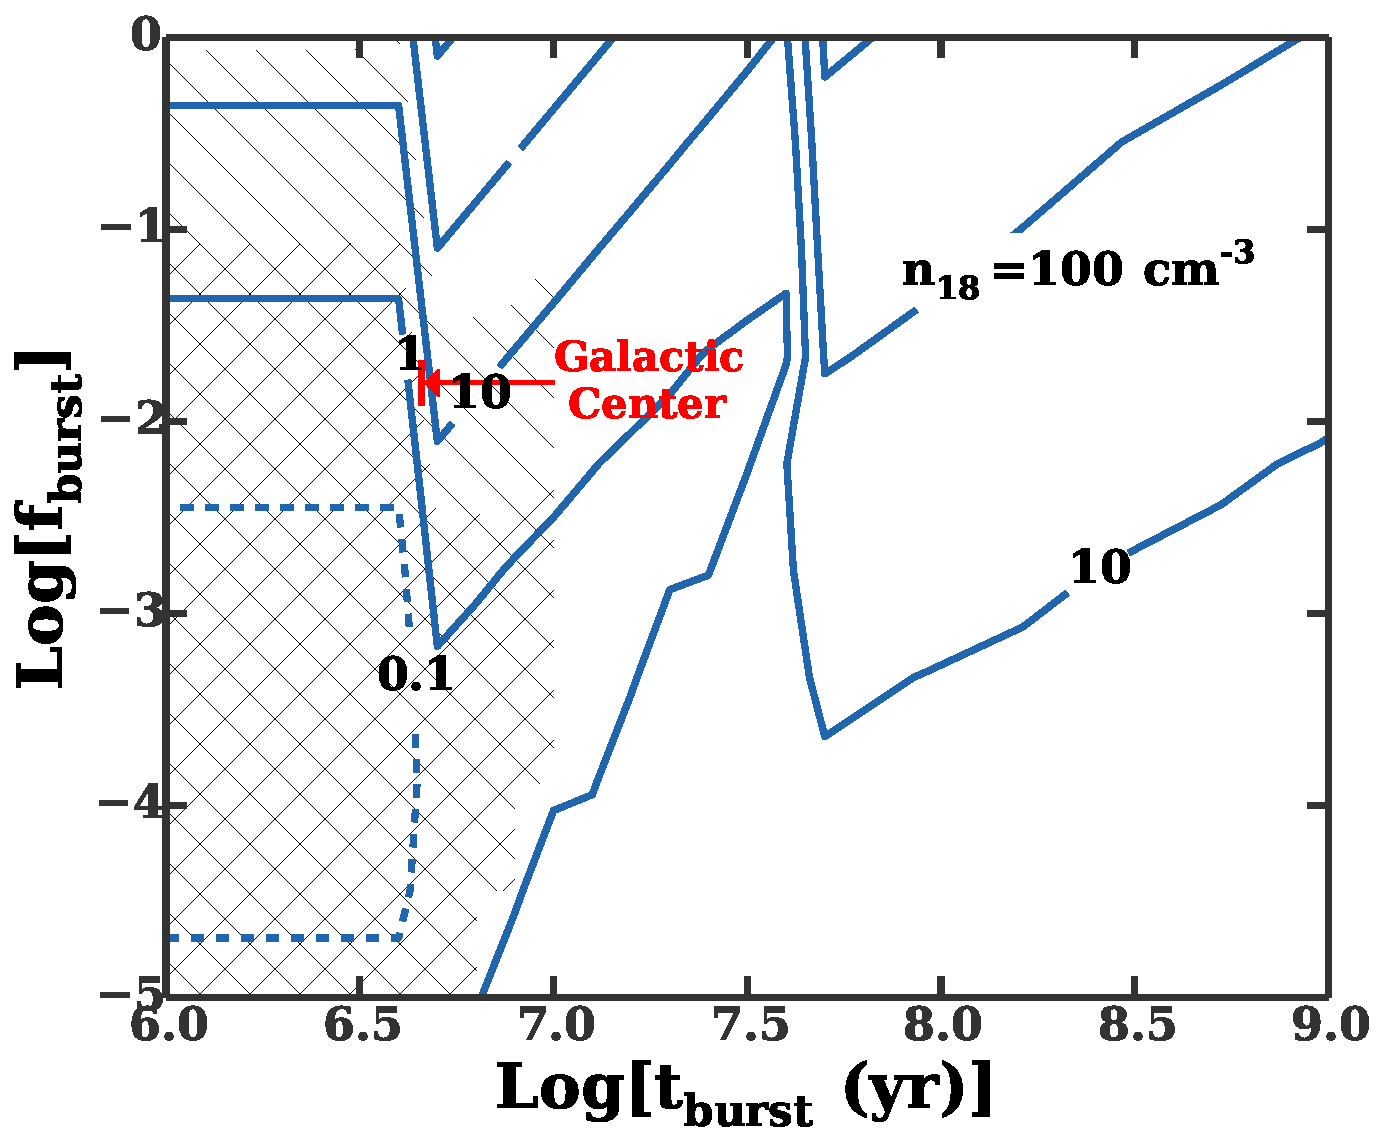
\includegraphics[width=8cm]{cnm_plot.pdf}
  \caption{\label{fig:param} Isocontours of $n_{18}$, the CNM density
    at $r = 10^{18}$ cm (blue lines), as a function of the stellar
    population in the galactic nucleus.  The star formation is
    parameterized assuming that a fraction $f_{\rm burst}$ of the
    stars form in a burst of age $t_{\rm burst}$, while the remaining
    stars formed a Hubble time ago.  We have assumed a black hole of
    mass $10^{7} \, \Msun$ and that both young and old stars possess a
    cusp-like density profile, which produces a gas density profile
    obeys $n \propto r^{-1}$.  Hatched areas indicate regions of
    parameter space where massive stars ($\gsim 15 \, \Msun$) dominate
    the gas heating rate, but less than one (doubly hatched) or less
    than ten (singly hatched) massive stars are present on average
    inside the nominal stagnation radius (eq.~\ref{eq:rs}).  In these
    regions of parameter space discreteness effects not captured by
    our formalism may be important. The red line shows the rough location of
    the Galactic Center in this parameter space.}
\end{figure}


% \begin{figure}
%   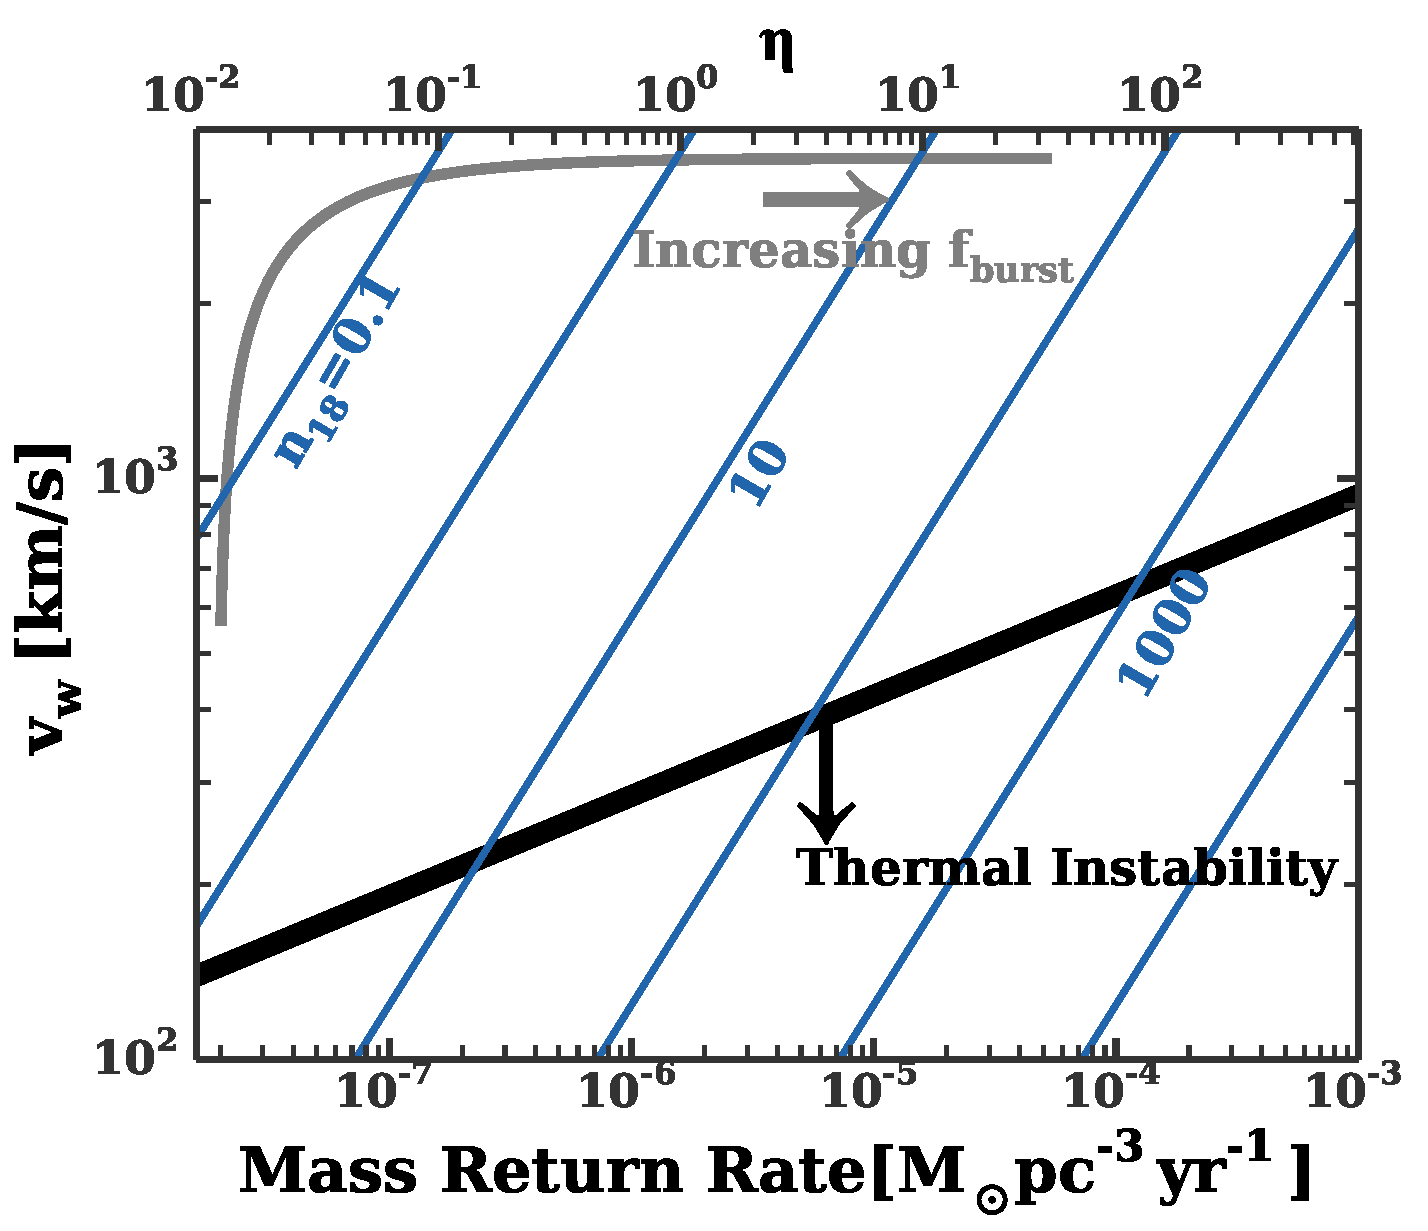
\includegraphics[width=8cm]{cnm_plot_2.pdf}
%   \caption{\label{fig:param2} $n_{18}$ as a function of the mass
%     return ($\eta$) and heating ($v_w$) parameters for a $10^7 \Msun$
%     black hole. We translate the gray line from Fig.~\ref{fig:param}
%     to this parameter space. $f_{\rm burst}$ increased in the direction
%     indicated by the gray arrow. As indicated by the black solid line,
%     the area below the black solid line is thermally unstable
%     (\textit{see text for discussion}).}
% \end{figure}

\subsection{Empirical Constraints on CNM Density}
\label{sec:empirical}

\subsubsection{Galactic center} 
Due to its proximity, it is possible to directly observe the gas
density distribution on parsec scales in the Galactic
center. \citet{Baganoff+2003} find that the hot, diffuse plasma within
10'' ($\sim \times 10^{18}$ cm) of Sgr A* has a root mean square
electron density of $\sim 26$ cm$^{-3}$, which implies a total number
density of $n\sim 50$ cm$^{-3}$. At the same time this estimate
includes regions closer to the center, where the gas density is
higher, so that the true number density at $10^{18}$ cm may be smaller
by a factor of $\sim 2$.

For the observed star formation rate of the Galactic Center (see
Fig. 14 of \citealt{Pfuhl+2015}), our formalism gives $n_{18}\sim 4-6$
cm$^{-3}$, where this range reflects the observational uncertainty in
the star formation history. Fig.~\ref{fig:param} shows the range
of two-burst star formation models, which produce heating and mass
return parameters equal to those derived from the full star formation
history of the Galactic Center. 

Our formalism give a somewhat lower value for the density in the
galactic center than that observed...{\bf AG discreteness effects and
  IMF. For example our stagnation radius is smaller than Quataerts
  since we do not use any detailed information about the stellar
  pop. So for example our stagnation radius is a factor of 4 further in.}

\subsubsection{Eddington ratio distribution}
We now translate observed constraints on the accretion
rate distribution of supermassive black holes into constraints on the
CNM density.  The accretion rate can be written as
\begin{equation}
\dot{M}_{\bullet} = f_{\rm in} 4 \pi r^2 \mu m_p n v,
\label{eq:mdot}
\end{equation}
where $n$ is the average density at radius $r$ and $f_{\rm in}$ is the
fraction of the large scale inflow which actually reaches small scales
and accretes onto the black hole.  Inside the sonic point the velocity
approaches the free-fall velocity, in which case
equation~\eqref{eq:mdot} becomes
\begin{equation}
  \dot{M}_{\bullet} = 1.1\times 10^{-5} \Mbh[,7]^{0.5} f_{\rm in}
  n_{18} \,\,\Msun {\rm yr}^{-1}.
\label{eq:mdot2}
\end{equation}
%
The corresponding Eddington ratio is
\begin{equation}
  \lambda\equiv L/L_{\rm Edd} = 4.8 \times 10^{-5}
  \left(\frac{\epsilon_{\rm rad}}{0.1}\right) \Mbh[,7]^{0.5} f_{\rm in}
  n_{18},
\label{eq:n18Edd}
\end{equation}
%
where $\epsilon_{\rm rad}$ is the radiative
efficiency. \citet{Kauffmann&Heckman2009} present distributions of the
OIII line luminosity, ${\rm L[OIII]}/\Mbh$ for a volume limited {\bf
  AG double check} sample of SDSS galaxies, where ${\rm
  L[OIII]}/\Mbh=1.7$ roughly corresponds to Eddington ratio of unity
(REF).  This bolometric correction maps the distribution of ${\rm
  L[OIII]}/\Mbh$ to a distribution of Eddington ratios
\citep{Kauffmann&Heckman2009}.

Equation (\ref{eq:mdot2}) provides a map between the Eddington ratio
and gas density $n_{18}$, provided that the radiative efficiency
$\epsilon_{\rm rad}$ and accretion efficiency $f_{\rm in}$ are known.
For the former we adopt the MHD shearing box results of
\citet{Sharma+2007}, who find (their Fig.~6)
\begin{align}
&\epsilon_{\rm rad} \simeq 
\begin{cases}
  0.03 \left(\frac{\dot{M}_{\bullet}}{10^{-4}\dot{M}_{\rm Edd}}\right)^{0.9} & \frac{\dot{M}_{\bullet}}{\dot{M}_{\rm edd}} \lsim 10^{-4} \\
 0.03 &  10^{-2} \gsim \frac{\dot{M}_{\bullet}}{\dot{M}_{\rm edd}}
 \gsim  10^{-4},
\end{cases}
\label{eq:efficiency}
\end{align}
where
\begin{equation} 
 \dot{M}_{\rm Edd} \equiv \frac{L_{\rm Edd}}{0.1 c^2} 
\end{equation}
%
and
there is a factor of $\sim$ 5 uncertainty in $\epsilon_{\rm rad}$ for
$\dot{M}/\dot{M}_{\rm Edd}\lsim 10^{-4}$ due to the dependence of the
results on uncertain microphysical parameters.  We linearly
interpolate between equation~\eqref{eq:efficiency} for
$\dot{M}/\dot{M}_{\rm Edd}<0.01$ and the standard thin-disk efficiency
of $\epsilon_{\rm rad}=0.1$ for $\dot{M}/\dot{M}_{\rm Edd}>0.1$.

\begin{figure}
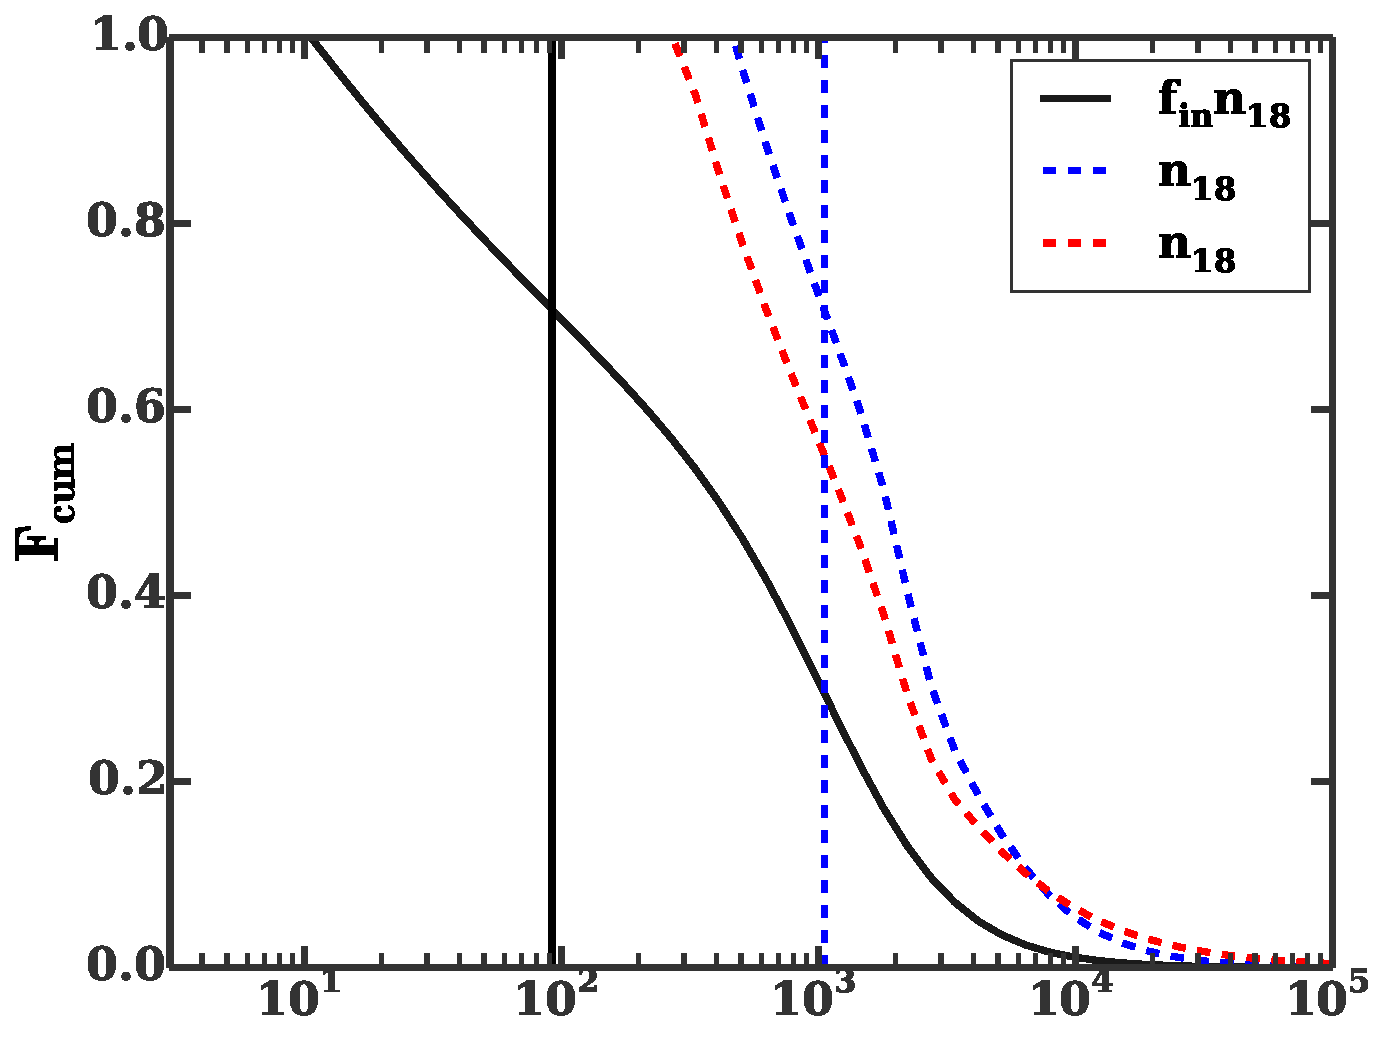
\includegraphics[width=8cm]{fcum_n18.pdf}
\caption{\label{fig:n18Cum} Cumulative distribution of $f_{\rm in}
  n_{18}$ for black holes with mass $\Mbh\simeq 10^{7} \Msun$ as
  inferred based on the distribution of measured Eddington ratios from
  \citet{Kauffmann&Heckman2009} {\it (solid black line)}. Here $f_{\rm
    in}$ is the ratio of the true accretion rate onto the black hole
  to the inflow rate of free-falling gas at $10^{18}$ cm.  A dashed
  blue line shows the corresponding cumulative distribution of
  $n_{18}$, obtained using values of $f_{\rm in}$ motivated by the
  simulations of \citet{Li+2013} (see text). The distribution of
  $f_{\rm in} n_{18}$ ($n_{18}$) is unreliable to the left of the
  solid black (dashed blue) vertical line.  Such low densities
  correspond to galaxies with small OIII luminosities, which could be
  the result of star formation instead of AGN activity.}
\end{figure}


Fig.~\ref{fig:n18Cum} shows the distribution of $f_{\rm in} n_{18}$
which results from combining the distributions of Eddington ratio from
\citet{Kauffmann&Heckman2009} with equations~\eqref{eq:n18Edd} and
~\eqref{eq:efficiency}.  It would at first appear that the absence of
galaxies with $f_{\rm in }n_{18} \lsim$ few cm$^{-3}$ places a lower
bound on $n_{18}$ of a few cm$^{-3}$ because $f_{\rm in} \le 1$.
However, because measurements of Eddington ratios below $\sim 10^{-3}$
(shown with a vertical line in Fig.~\ref{fig:n18Cum}) are not reliable
(T.~Heckman, private communication), this allows a significant fraction
($\sim 30\%$) of galaxies to have lower gas densities.

To obtain the cumulative distribution of $n_{18}$ requires an
additional prescription for $f_{\rm in}$.  We use the results of
\citet{Li+2013}, who perform two-dimensional hydrodynamical
simulations of axisymmetric rotating accretion flows.  They find that
when the inflow rate on large scales is highly sub-Eddington
($\dot{M}/\dot{M}_{\rm Edd} \lsim 10^{-4}$), cooling is inefficient
and $f_{\rm in}\sim 0.01$. On the other hand, when
$\dot{M}/\dot{M}_{\rm Edd}\gsim 10^{-2}$, $f_{\rm in}$ approaches
unity.  We use $\dot{M}_{\bullet}/\dot{M}_{\rm Bondi}$ in their Figure
6 for $f_{\rm in}$.\footnote{\citet{Li+2013} employ an alpha viscosity
  prescription with $\alpha=0.01$.  A higher value of $\alpha$ would
  likely increase the accretion fraction $f_{\rm in}$, thus decreasing
  our estimates of $n_{18}$ in a systematic way.}  With this choice we
find that only a third of nuclei have $n_{18}>2\times 10^{3}$
cm$^{-3}$ and only 6\% have $n_{18}>10^{4}$ cm$^{-3}$.  We note,
however, that existing candidate tidal disruption flares show little
or no evidence for AGN emission lines (e.g. \citealt{van-Velzen+2011,
  Arcavi+2014}), making them unlikely to reside in the high density
tail of the $n_{18}$ distribution.

%Two potential complications to keep in mind are (i) clumpiness of the
%CNM and (ii) anisotropy. The distributions above are distributions of
%the {\it average} $n_{18}$.  Most likely, some of the nuclear gas in a
%low density hot phase, while the rest is in high density cold
%clumps/filaments.  However, while the jet is relativistic the
%light curve of a jet propagating through a clumpy medium will differ
%little from that of a smooth medium with the same average
%density. Even in the late stages when the jet becomes non-relativistic
%clumps will only make a difference if the size of the clumps is
%comparable to the size of the jet {\bf AG include some refs here}.
One potential complication is that the CNM could be distributed
anisotropically around the black hole.  The cold phase could be
concentrated in a ring-like structure, similar to the cirumnuclear
ring surrounding SgrA$^{*}$ (e.g.~\citealt{Lau+13}).  Anisotropies may
also present in the hot phase, for instance due to low density bubbles
inflated by the AGN.  However, insofar as the angle of the TDE jet is
large compared to these features, the quantitative impact on the radio
flux is unlikely to be large.

%For instance, X-ray observations of the nuclei of massive elliptical galaxies show densities of density on scales of $\sim
%100$ pc is $\gsim 0.1$ cm$^{-3}$

%For instance, \citet{Russell+2013} use X-ray observations to measure
%gas density and temperature profiles for a sample of massive elliptical galaxies. The measured electron density on scales of $\sim
%100$ pc is $\gsim 0.1$ cm$^{-3}$. Note that the gas density at 100 pc
%would be irrelevant for a TDE jet, but we would not expect the gas
%density to be decreasing towards the galactic center in a steady
%state.  We note that massive black holes in the \citet{Russell+2013}
%sample, with $\Mbh\sim 10^{9} \Msun$, whereas black holes tidal
%disruption events would have $\Mbh\lsim 10^8 \Msun$. This is because
%more massive black holes would not be able to disrupt (main sequence)
%stars.

%In this scenario, the
%some fraction of jets would likely be stifled by the very dense
%ring. However, such a ring would not block all jet propagation
%directions.

The empirical estimates in this section nicely complement our analytic
results.  The accretion rates of black holes are particularly are
particularly challenging to measure for quiescent nuclei.  However,
such cases, in which AGN feedback is minimal, are precisely the regime
where our analytic estimates are the most trustworthy, providing a
lower density floor of $n_{18} \sim 0.5$ cm$^{-3}$.

% On the other hand, the analytic estimates are specific to
% the hot phase of gas. The Eddington ratio distribution probes the
% average density (including any cold clumps). The
% distribution of Eddington ratios gives us confidence in our high
% density limit ($\sim 1000$ cm$^{-3}$).



% We show a comparison of this modified 1D approach with the true 2D
% result in Figure~\ref{fig:1D2DB}, for $n_{18}=60$ and $n_{18}=2000$
% and $E_{\rm ISO}=4 \times 10^{54}$ ergs. For $n_{18}=2000$ the
% agreement is excellent, while for $n_{18}=60$ the 1D models still
% over-predict still over-predict the flux at times after the peak of
% the light curve.



\begin{table}
\begin{threeparttable}
  \caption{\label{tab:jetParams} Summary of parameters for grid of on
    axis jet simulations.}
  \begin{tabular*}{0.95\columnwidth}{lll}
    Fast component ($\Gamma=10$) & Fiducial value & Other values \\ 
    \hline
    $[\theta_{\rm min}$, $\theta_{\rm max}]$ & [0, 0.1] radians & \\
    $E_{\rm ISO}/10^{54}$ erg & 4  & 0.04, 0.4\\
    $E/10^{54}$ erg & 0.02 & \\
    \hline 
    Slow component ($\Gamma=2$)\\
    $[\theta_{\rm min}$, $\theta_{\rm max}]$ & [0.1, $\pi/2$] radians
    & \\
    $E_{\rm ISO}/10^{54}$ erg & $4.7$ & 0.047, 0.47 \\
    $E/10^{54}$  erg & $0.47$ erg & \\
    \hline
    Micro-physical parameters\\
    $\epsilon_e$ & 0.1 &  0.05, 0.2\\
    $\epsilon_b$ & 0.002 & 0.001, 0.005\\
    $p$ & 2.3\\
    \hline 
    Nuclear gas density \\
    $n_{18}$ [cm$^{-3}$] & 60 & 2, 11, 345, 2000
  \end{tabular*}
% \begin{tablenotes}
% \item $^{\dagger}$  Additional values of physical parameters we tried.
% \end{tablenotes}
\end{threeparttable}
\end{table}


\section{Synchrotron Radio Emission}

\label{sec:results}
\subsection{Numerical Jet Simulation}
\label{sec:numerical}
We calculate synchrotron radio emission from the TDE jet propagating
through and shocking the CNM across the physically plausible range of
nuclear gas densities.  The jet-CNM interaction is simulated in both
one and two dimensions, and the resulting synchrotron emission is
computed as described in \citet{Mimica+2015}.  {\bf BDM: slightly more
  detail about numerical procedure}

For the jet structure we adopt the preferred two-component model for
SwJ1644 from \citet{Mimica+2015}, corresponding to a fast, inner core
with Lorentz factor $\Gamma = 10$, surrounded by a slower, $\Gamma=2$
outer sheath.  For our 2D simulations the fast inner core spans an
angular interval $0-0.1\ {\rm radians}$, while the slow outer sheath
extends from $0.1\ {\rm radians}$ to $0.5\ {\rm rad}$
(\citealt{Mimica+2015}).  The time dependence of the jet kinetic
luminosity is given by
\begin{equation}\label{eq:lum}
L_{\rm j, ISO}(t) = L_{j,0}\max\left[1, (t/t_0)\right]^{-5/3}
\end{equation}
%
where the $t_0 = 5\times 10^5$ s is the duration of peak jet power and
approximately corresponds to the duration of the peak non-thermal
X-ray emission of SwJ1644.  Integrating equation~\ref{eq:lum} from $t
= 0$ to $\infty$ gives the isotropic equivalent energy of the jet,
$E_{\rm ISO}$, where $L_{j,0}=0.4\, E_{\rm ISO}/t_0$.  The ratio of
the true (beaming-corrected) energy of the fast component is fixed to
be 4\% of that in the slow component (\citealt{Mimica+2015}).

For our 1D simulations, we modify the geometry of the slow sheath to
better reproduce the results of the 2D simulations.  Although in out
2D models the sheath is injected within a relatively narrow angular
interval, at late stages of evolution the bow shock created by the
jet-CNM interaction spans a much larger range of angles due to
laterial spreading, i.e. the slow component becomes almost isotropic
in 2D \citep[bottom two panels of Fig.~8 in][]{Mimica+2015}. To
account for this in our 1D simulations, we instead take the slow
component to extend from 0.1 to $\pi/2$ radians.

Fig.~\ref{fig:1D2DB}, shows a comparison of light curves from this
modified 1D approach and the 2D simulations. Although, the slow
component in the 1D simulations is initially much broader 2D
simulations, the 1D results and 2D results are quite close at high
densities ($n_{18}=2000$ cm$^{-3}$). This is because the slow
component rapidly spreads out and isotropizes in 2D. The agreement is
not as good for $n_{18}=60$ cm$^{-3}$, for which the 1D calculation predict
systematically higher luminosities. Nonetheless, using a broadened
slow component in 1D leads to better agreement with 2D results {\bf
  AG: Is this actually true for n18=60?}.

% Fig~\ref{fig:components}, which shows the relative contributions of
% the fast and slow components to the 5 GHz light curve of a $5 \times
% 10^{53}$ erg jet for different ambient gas densities. For
% $n_{18}=2000$ cm$^{-3}$, the slow component dominates for nearly all
% times.  For $n_{18}=2$ cm$^{-3}$, the fast component dominates at
% early times and at the peak of the light curve, while the slow
% component dominates after $\sim$1 year. In general, the fast component
% is more important for early times, higher frequencies and smaller
% ambient gas densities.

\begin{figure}
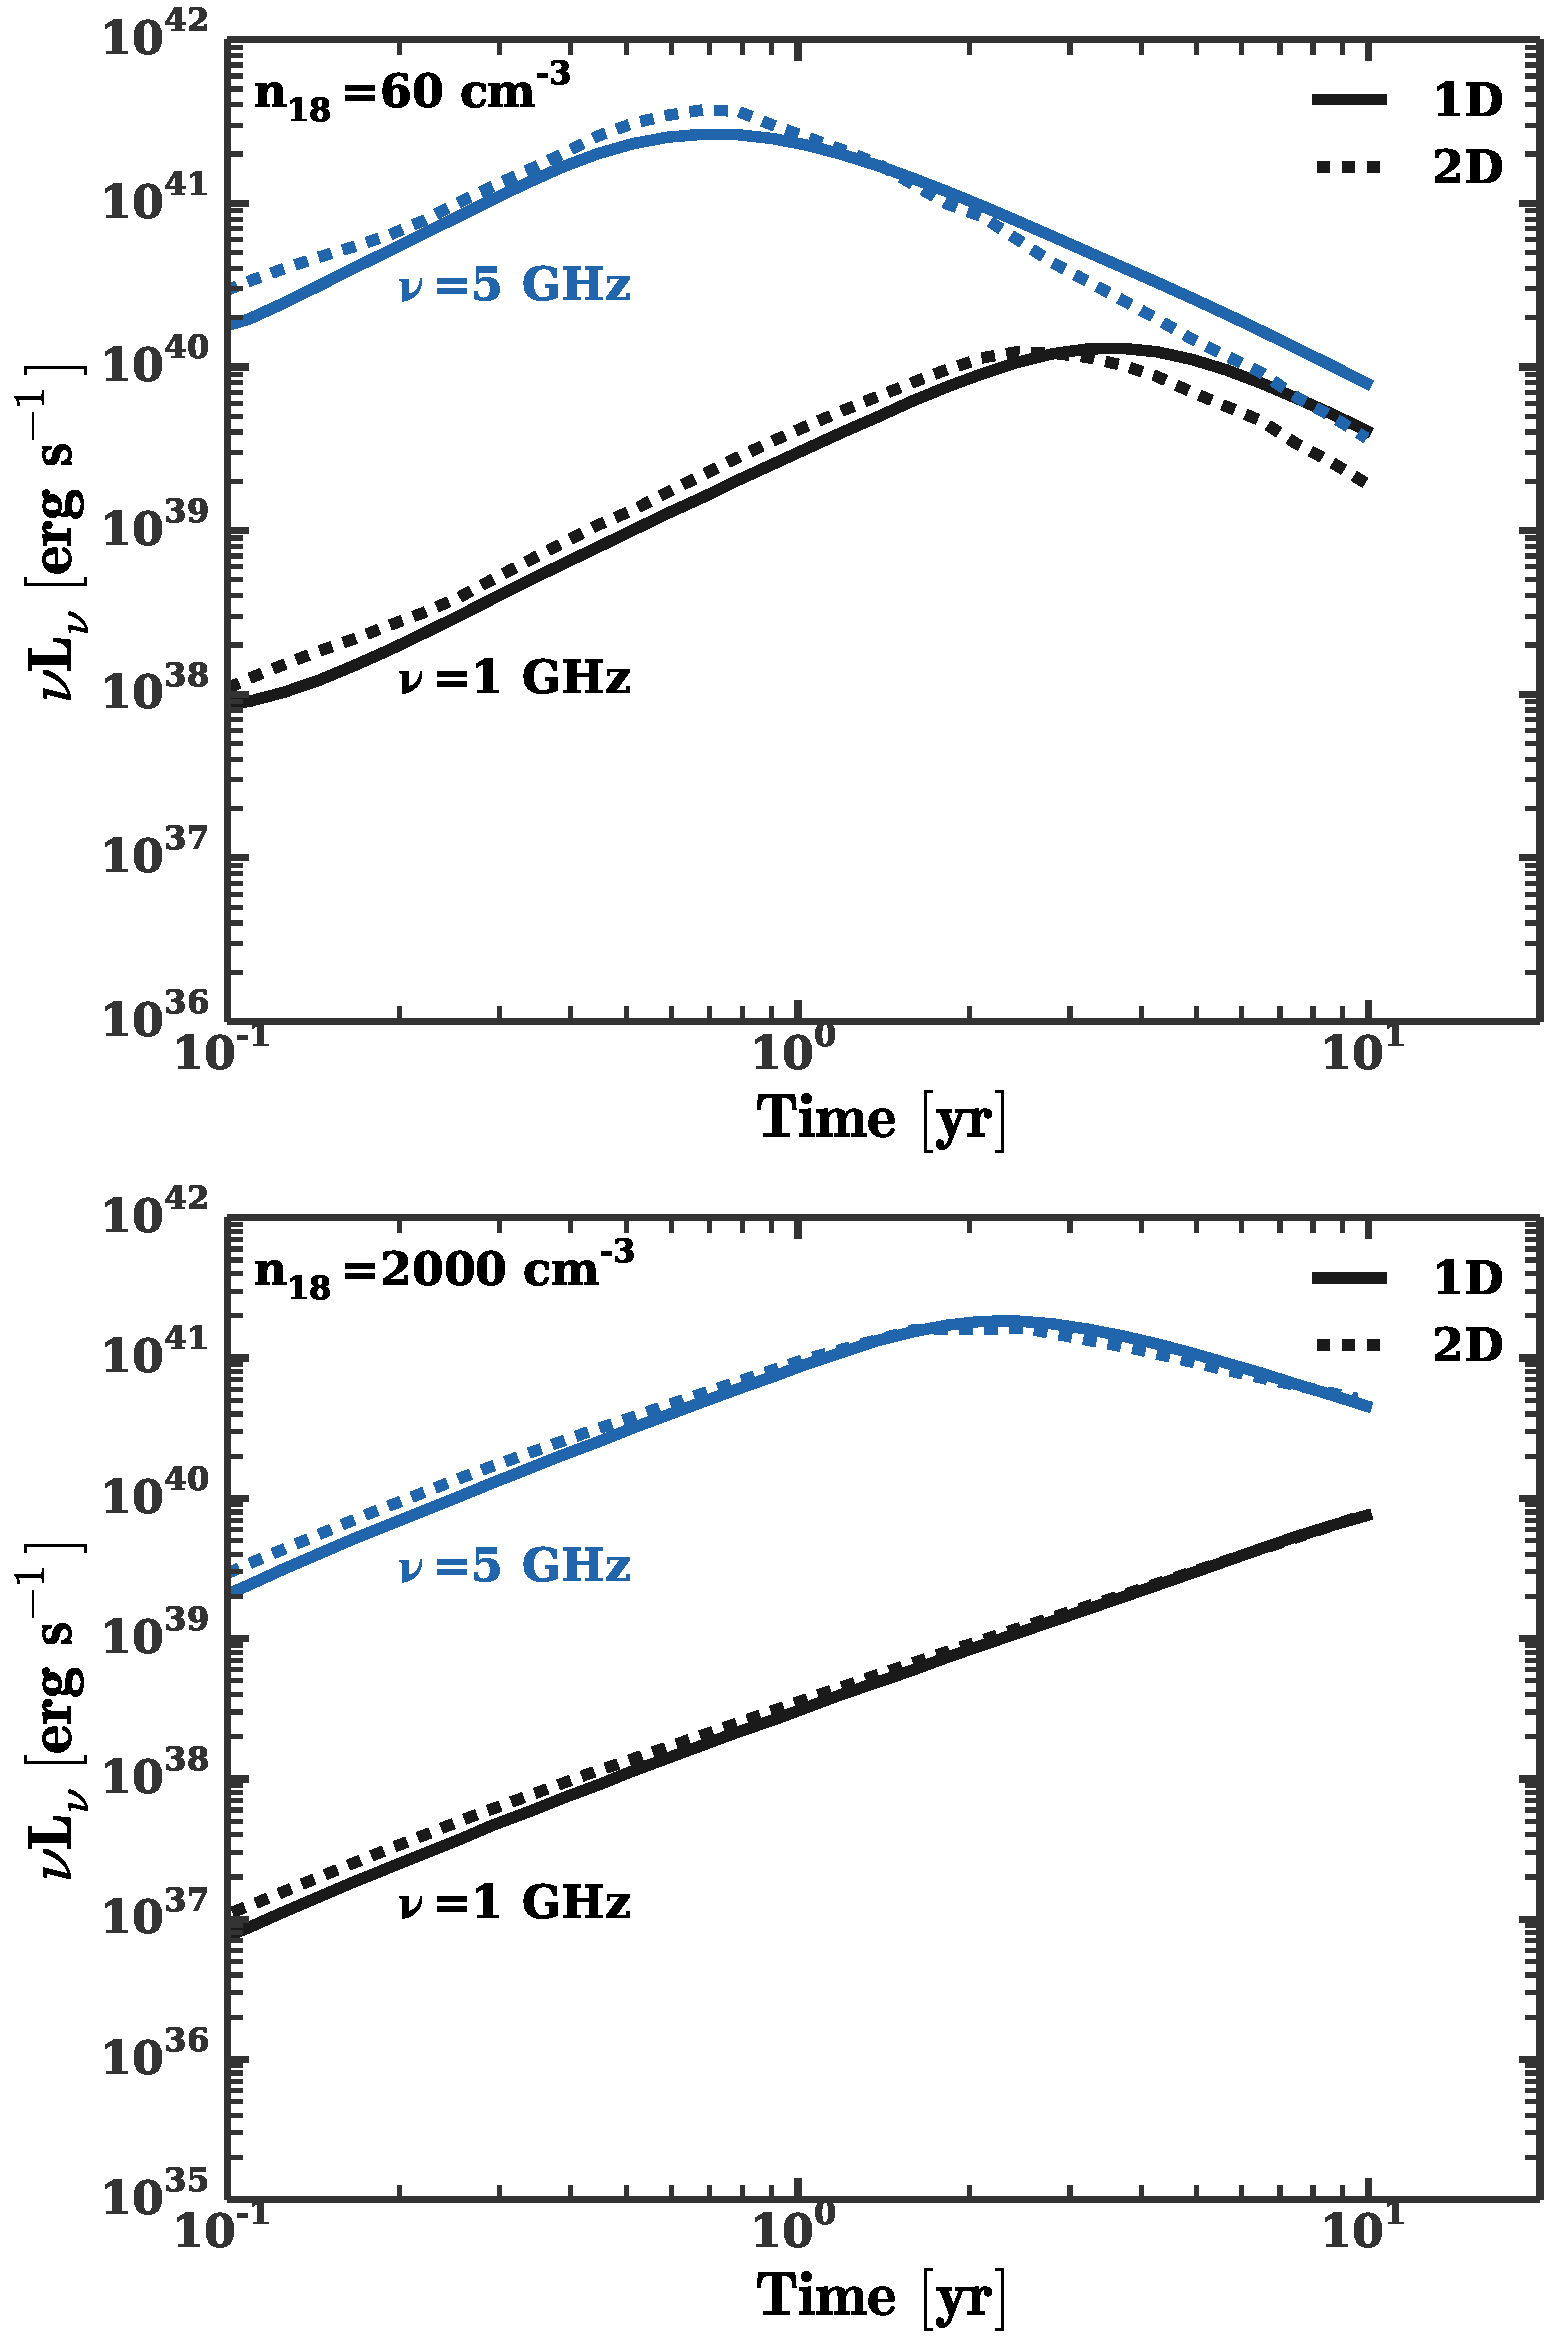
\includegraphics[width=8cm]{1d_2d.pdf}
\caption{\label{fig:1D2DB} Comparison of light curves from 1D and 2D
  simulations for $n_{18}=60$ cm$^{-3}$ (top) and $n_{18}=2000$
  cm$^{-3}$ (bottom) for frequencies of 1 GHz and 5 GHz and an
  observer angle of 0.8 radians to the jet axis. We assume that the
  gas density $n\propto r^{-1}$ for $n_{18}=2000$ cm$^{-3}$, but take
  $n\propto r^{-1.5}$ for $n_{18}=60$ cm$^{-3}$ for computational
  convenience--this model was previously computed in
  \citet{Mimica+2015} and 1D results suggest that the density slope
  would have minimal impact on the results (see
  $\S$~\ref{sec:profileComp})}.
\end{figure}

\subsection{Light curves}
\label{sec:lightcurves}
In this section, we investigate the effects of the gas density
profile, the jet energy, and observer viewing angle on the observed
synchrotron radio light curve. 

\subsubsection{Analytic results}
The dependence of synchrotron peak luminosity and peak time on ambient
gas density and jet parameters can be derived analytically by
calculating the synchrotron radiation from the shocked slab of gas
behind a self-similarly expanding blast wave. This was done in
\citet{Leventis+2012}. The relevant results from this work are
summarized in Appendix~\ref{app:analyt}. Equation~\ref{eq:peakLumGen}
shows the dependence of the peak luminosity slow component on jet
parameters and ambient gas density. Substituting in our fiducial
values for power law slopes of the gas density profile and energy
distribution of accelerated electrons ($p$) gives

\begin{align}
\nu L_{\nu, p}&=
\begin{cases}
  4.9\times 10^{40} \left(\frac{E}{10^{54} {\rm ergs}}\right)^{0.59}
  \left(\frac{\epsilon_e}{0.1}\right)^{1.3}
  \left(\frac{\epsilon_b}{0.002}\right)^{0.825}\\
  \left(\frac{\nu_{\rm obs}}{5 {\rm GHz}}\right)^{0.35} n_{18}^{1.24} 
  {\rm erg \, s^{-1}} & {\rm Case \,1}\\\\
 1.1 \times 10^{42}  \left(\frac{E}{10^{54} {\rm ergs}}\right)^{0.87}
  \left(\frac{\epsilon_e}{0.1}\right)^{0.61}
  \left(\frac{\epsilon_b}{0.002}\right)^{0.26}\\
  \left(\frac{\nu_{\rm obs}}{5 {\rm GHz}}\right)^{2.01} n_{18}^{-0.14}
  {\rm erg\, s^{-1}} & {\rm Case \,2}
\end{cases}
\label{eq:peakLum}
\end{align}
%
Case 1 would be relevant for a low density medium, in which the jet is
optically thin at the deceleration time. In this case, the peak
luminosity is quite sensitive to density. Case 2 would be relevant for
a high density medium, in which the jet is optically thick at the
deceleration time. In this case, the peak luminosity is only weakly
dependent on the ambient gas density. The normalizations for Case 1
and Case 2 are chosen to match our numerical results at low and high
densities respectively.

Equation~\eqref{eq:tpeakGen} gives the peak time for the slow
component. Substituting in our fiducial values for power law slopes of
the gas density profile and energy distribution of accelerated
electrons, gives


\begin{align}
t_p=
\begin{cases}
  t_1 E_{54}^{0.5} n_{18}^{-0.5} & {\rm Case \, 1}\\\\
  t_2 \left(\frac{E}{10^{54} {\rm ergs}}\right)^{0.32}
  \left(\frac{\epsilon_e}{0.1}\right)^{0.45}
  \left(\frac{\epsilon_b}{0.002}\right)^{0.37}\\
  \left(\frac{\nu_{\rm obs}}{5 {\rm GHz}}\right)^{-1.1} n_{18}^{0.4} &
  {\rm Case \, 2}
\end{cases}
\label{eq:peakTime}
\end{align}
%
where $t_1$ and $t_2$ are constants. In general, the light curve of a
higher energy jet will peak later than the light curve for a low
energy jet. The scaling with density is more complicated: if the
emitting region is optically thick at the deceleration time (``Case
2''), a higher ambient density results in a later peak time. The peak
occurs when the self-absorption frequency crosses through the
observing band and this occurs later for higher ambient gas
densities. Otherwise, the peak time will scale as the deceleration
time, and a larger ambient gas density will result in a later peak
(``Case 1'').


\subsubsection{Numerical results}
The left-hand panel of Fig.~\ref{fig:lightcurves} shows example light
curves from both 1D and 2D simulations of $5\times 10^{51}$ erg and
$5\times 10^{53}$ erg jets going through $n\propto r^{-1}$ density
profiles with different normalizations. The peak luminosity is
virtually independent of density.  This consistent with our analytic
expectations for high densities and low frequencies: the emission is
dominated by the slow component, which is optically thick at the
deceleration time. In this case the peak luminosity is virtually
independent of density (``Case 2'' in eq.~\ref{eq:peakLum}). For high
frequencies and small densities, the peak luminosity of the slow
component falls off (see right-hand panel of
Fig.~\ref{fig:lightcurves}). Coincidentally, the fast component just
compensates for this decline in the slow component luminosity, so the
total peak luminosity is nearly independent of density across the
parameter space. In fact, the ``Case 2'' peak luminosity in
equation~\ref{eq:peakLum} provides a good approximation for the total
peak luminosity for a fixed value of $n_{18}=2000$ cm$^{-3}$.

In general, the peak time is a decreasing function of the ambient gas
density. The peak occurs after the deceleration time when the emitting
region transitions from optically thick to optically thin. This
transition occurs later for larger ambient gas densities. Note,
however, that at 30 GHz, the slow component light curve peaks later
for $n_{18}=2$ than for $n_{18}=60$. This is the optically thin limit
(``Case 1'' in eq.~\ref{eq:peakTime}), in which the peak time scales
with the deceleration time, which is an increasing function of the
ambient gas density (see eq.~\ref{eq:tdec}).

\begin{figure*} 
  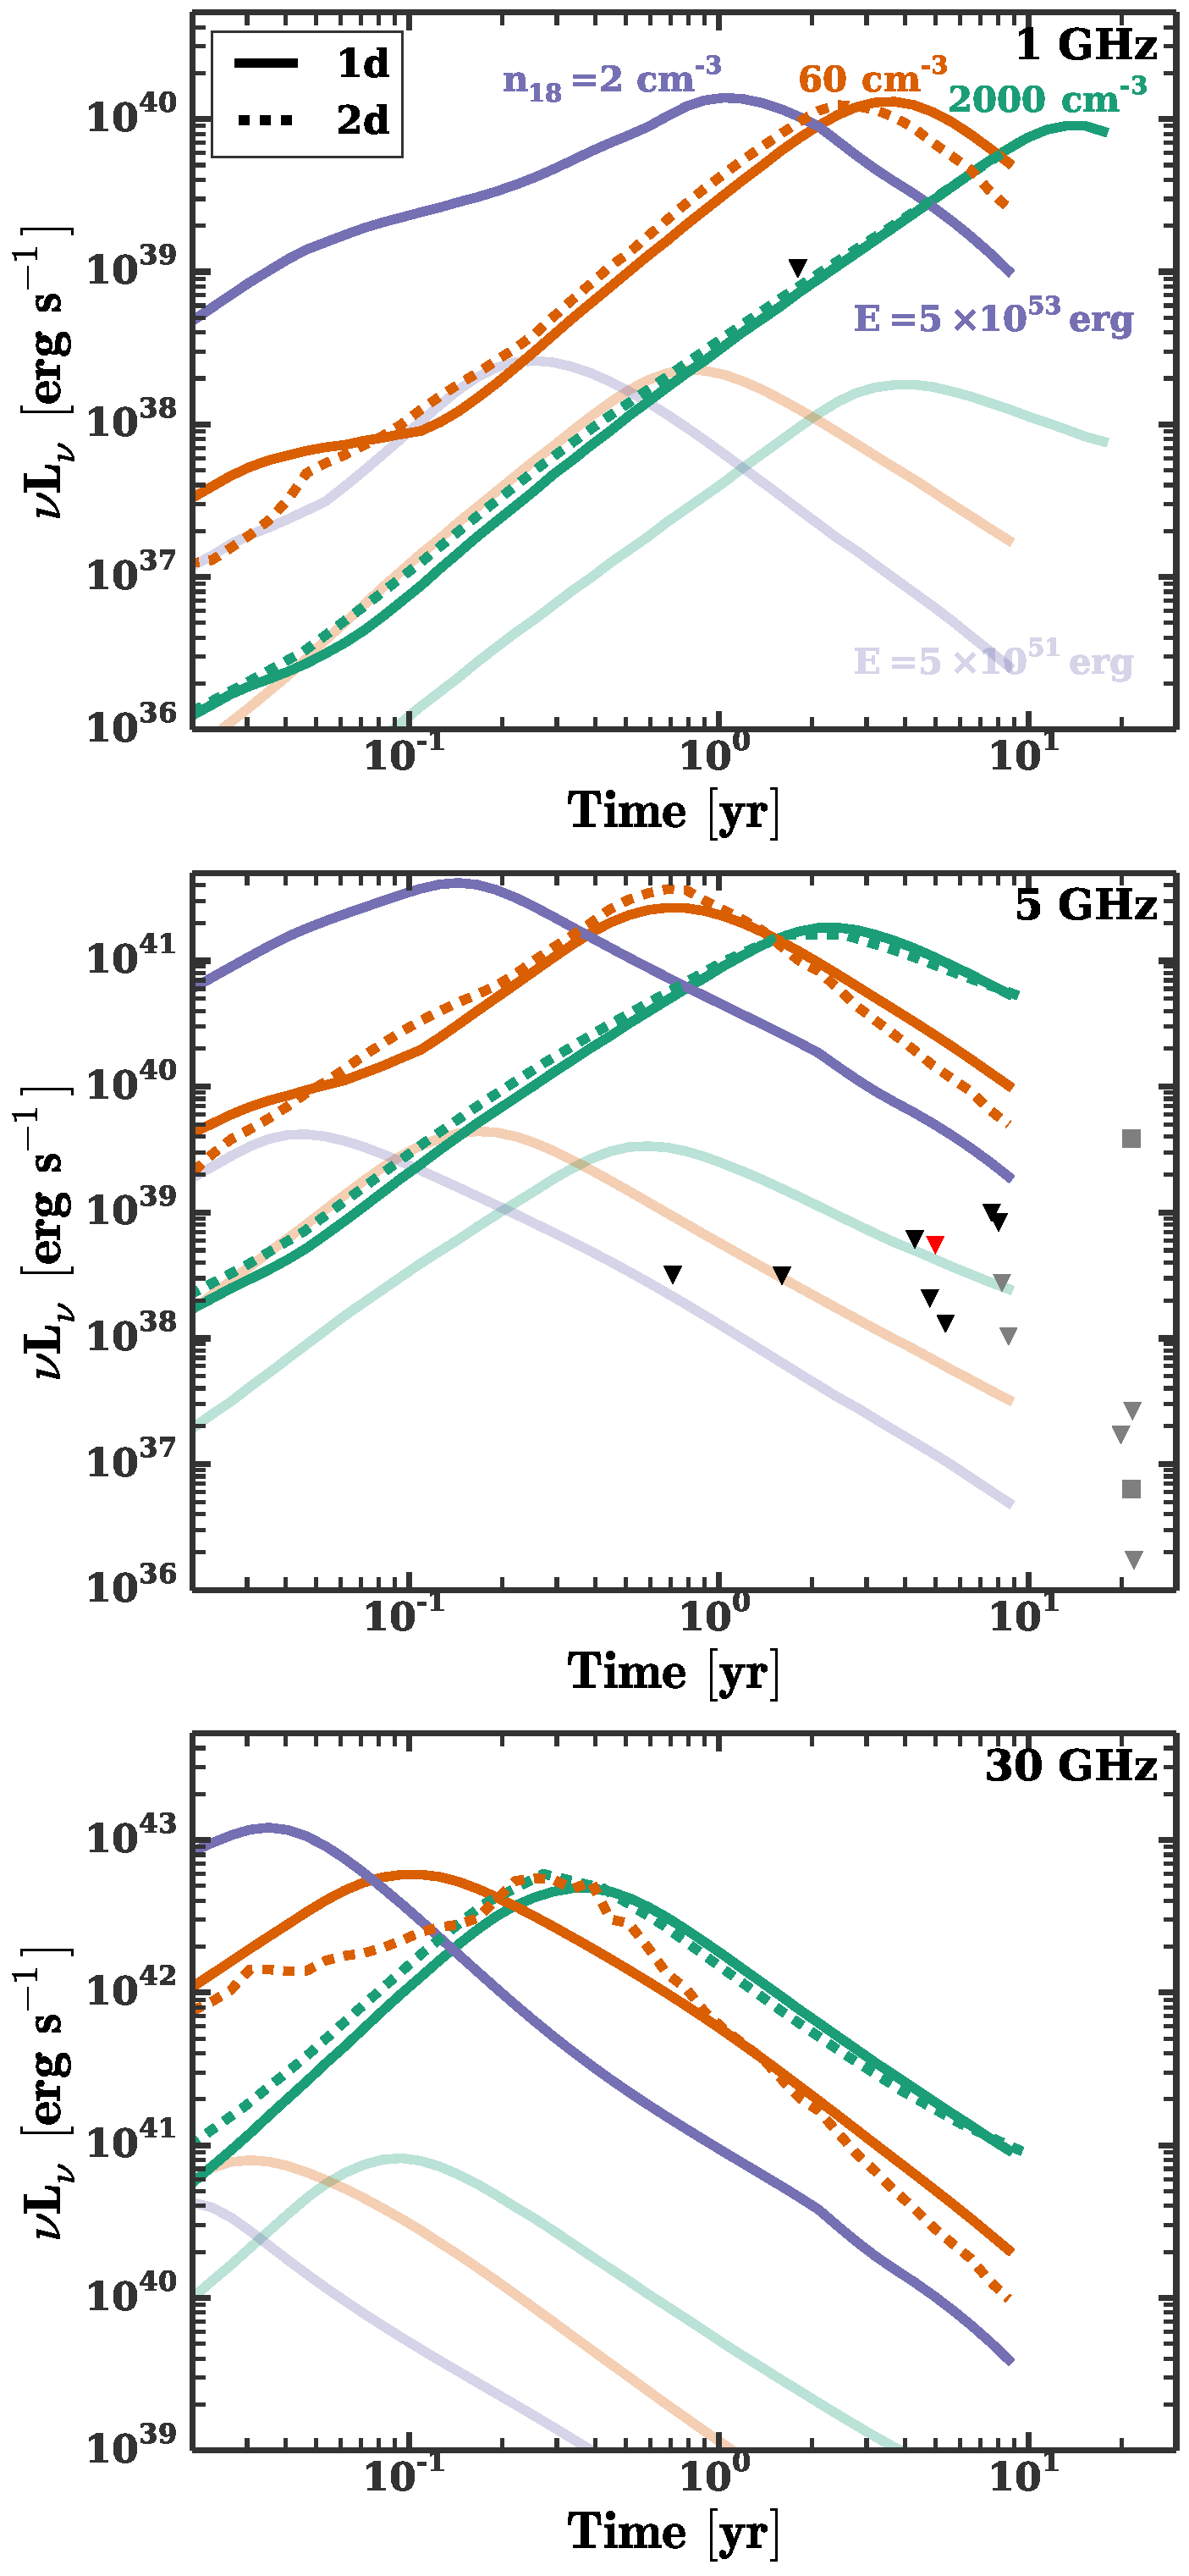
\includegraphics[width=8cm]{lightcurves.pdf}
  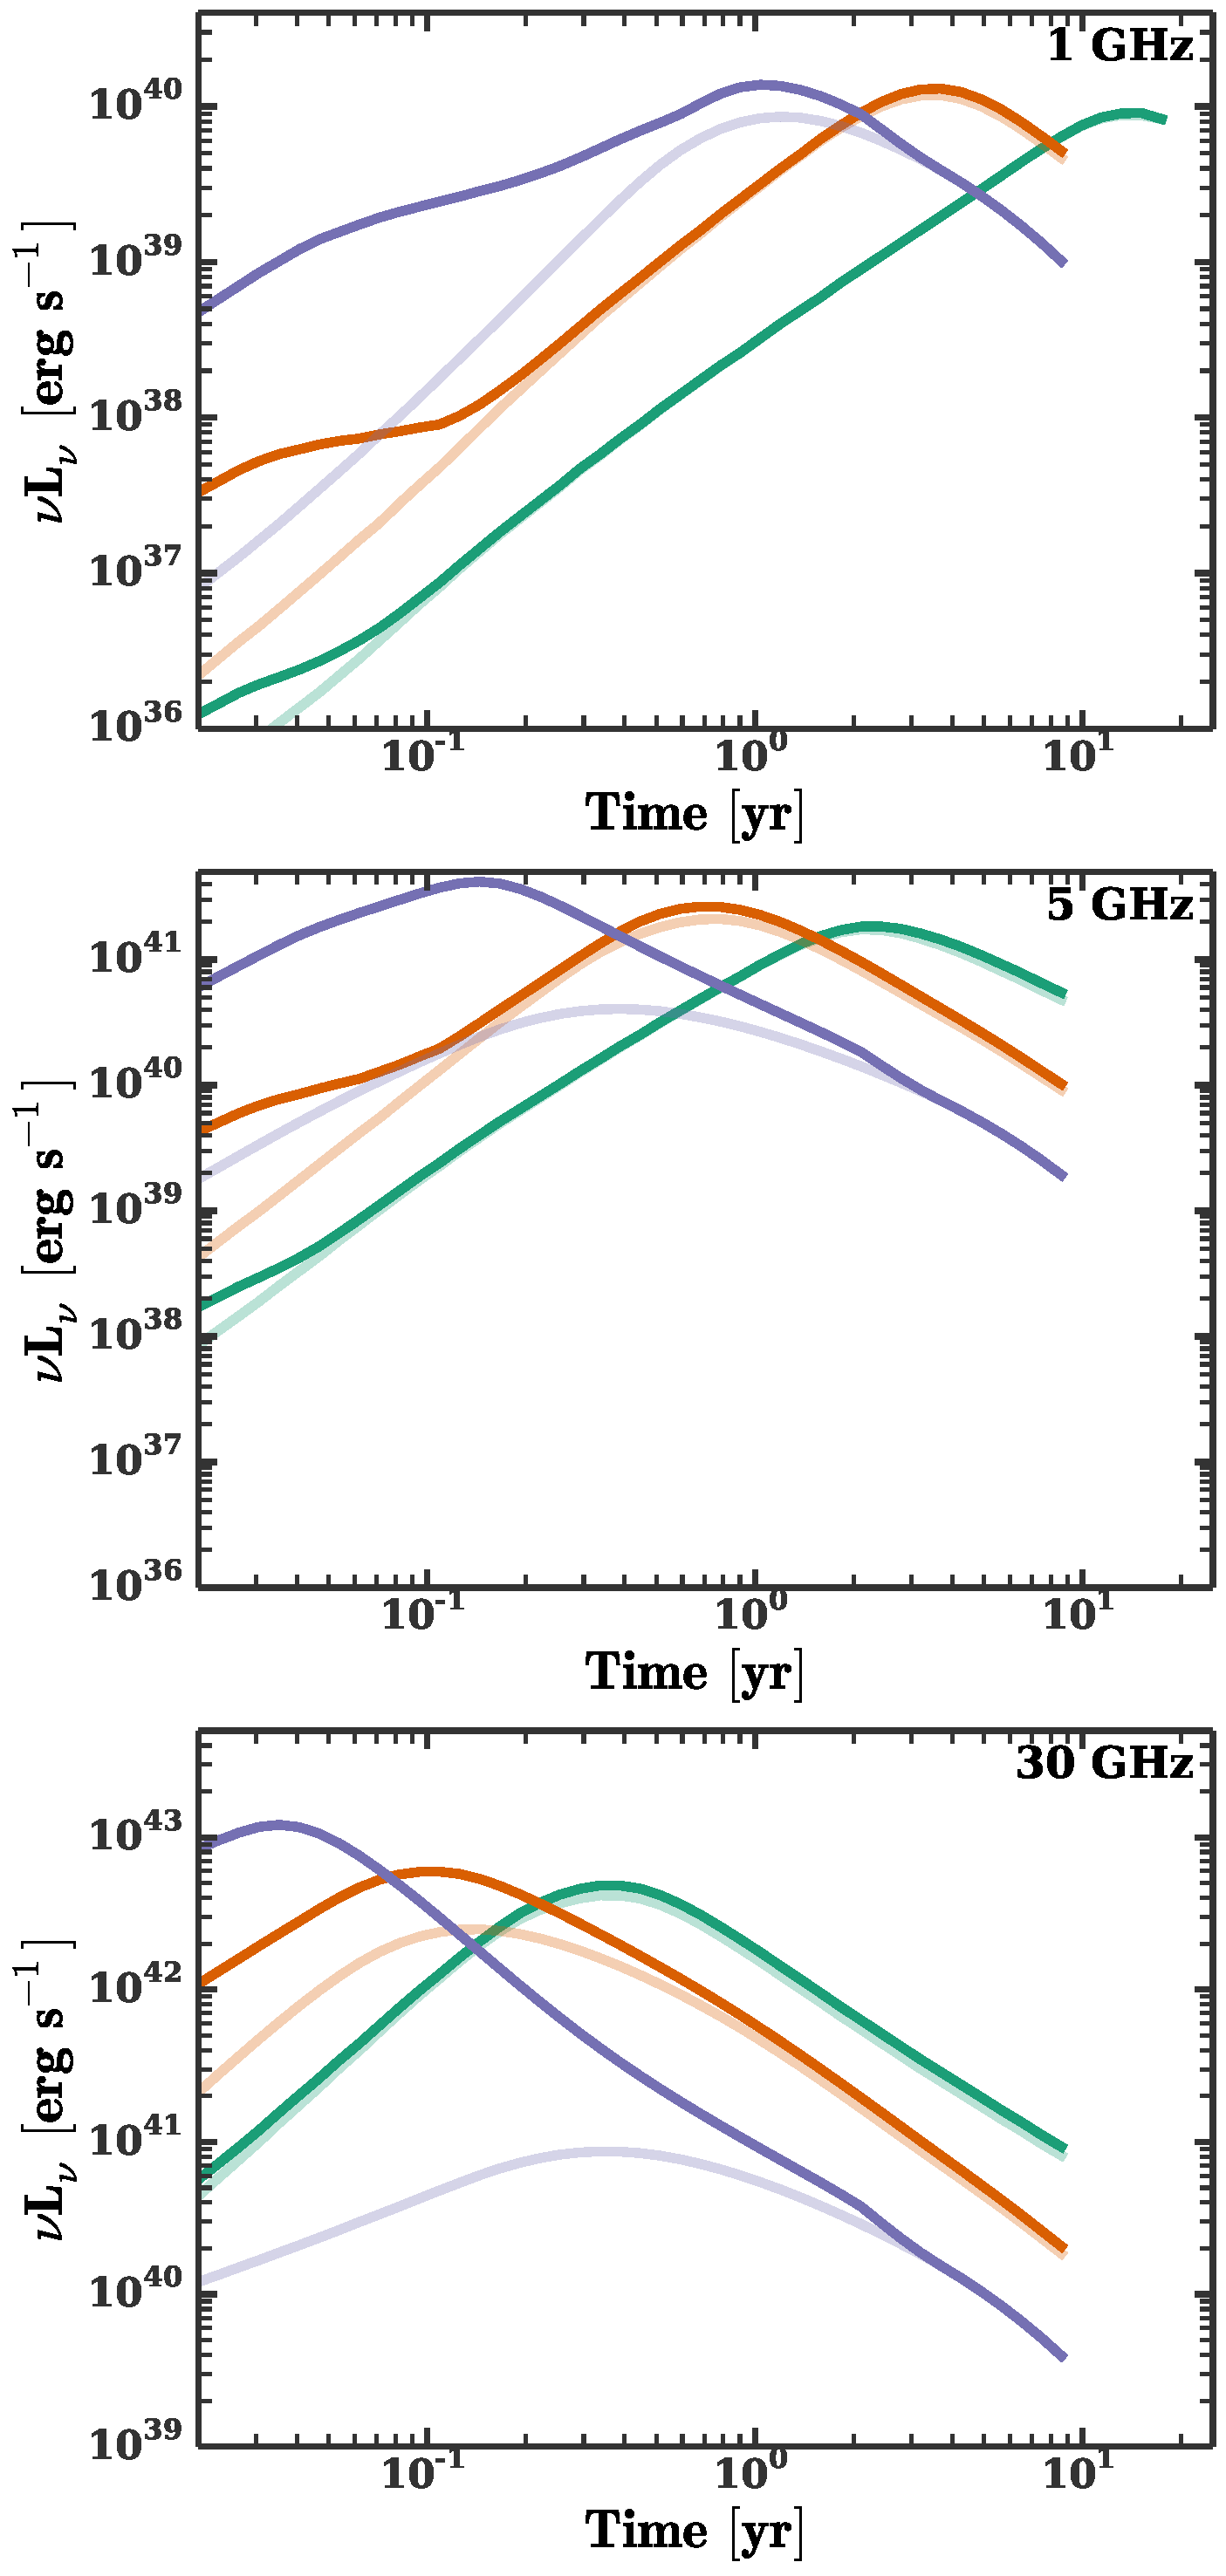
\includegraphics[width=8cm]{lightcurves_comp.pdf}
  \caption{\label{fig:lightcurves} \textit{Right-hand panel:} On-axis
    ($\theta_{\rm obs}=0$) radio light curves for jet energies of
    $5\times 10^{53}$ ({\it opaque}) and $5\times 10^{51}$ erg
    ({\it translucent}) and three different values of n$_{18}$: 2, 60,
    and 2000.  Solid lines correspond to the light curves from 1D jet
    simulations. When available ($n_{18}=60$ cm$^{-3}$ and
    $n_{18}=2000$ cm$^{-3}$), we have plotted light curves from the 2D
    jet simulations as dashed lines. Note we use $n\propto r^{-1}$ for
    $n_{18}=$ 2 and 2000, but $r^{-1.5}$ for $n_{18}=60$ cm$^{-3}$, as
    this model had already been computed and since the 1D results
    suggest that the density slope will have minimal impact on the
    results (see $\S$~\ref{sec:profileComp}).  Radio upper limits and
    detections are shown as black/gray triangles and squares
    respectively (compiled in Table 1 of \citealt{Mimica+2015}). The
    single upper limit in the top panel corresponds to 1.4 GHz. Gray
    triangles and squares in the middle panel indicate upper limits
    and detections at 3.0 GHz, while black triangles indicate upper
    limits at 5.0 GHz. \textit{Left-hand panel:} Total ({\it opaque})
    and slow component ({\it translucent}) on-axis light curves for a
    $5\times 10^{53}$ erg jet.}
\end{figure*}


 \subsubsection{Effects of viewing angle}
 Fig.~\ref{fig:onOff} shows a comparison of light curves for observers
 aligned with the jet axis (on-axis) and an angle of 0.8 radians off
 of the jet axis.  For $n_{18}=2000$ cm$^{-3}$ the light curves differ
 little.  For $n_{18}=60$ cm$^{-3}$ off-axis luminosity is lower by a
 factor of a few before and near the peak. However, for late times the
 off- and on-axis light curves are quite similar. This is as expected,
 at late times the jet becomes more isotropic, which means the viewing
 angle has relatively little effect on the observed light curve.

\begin{figure}
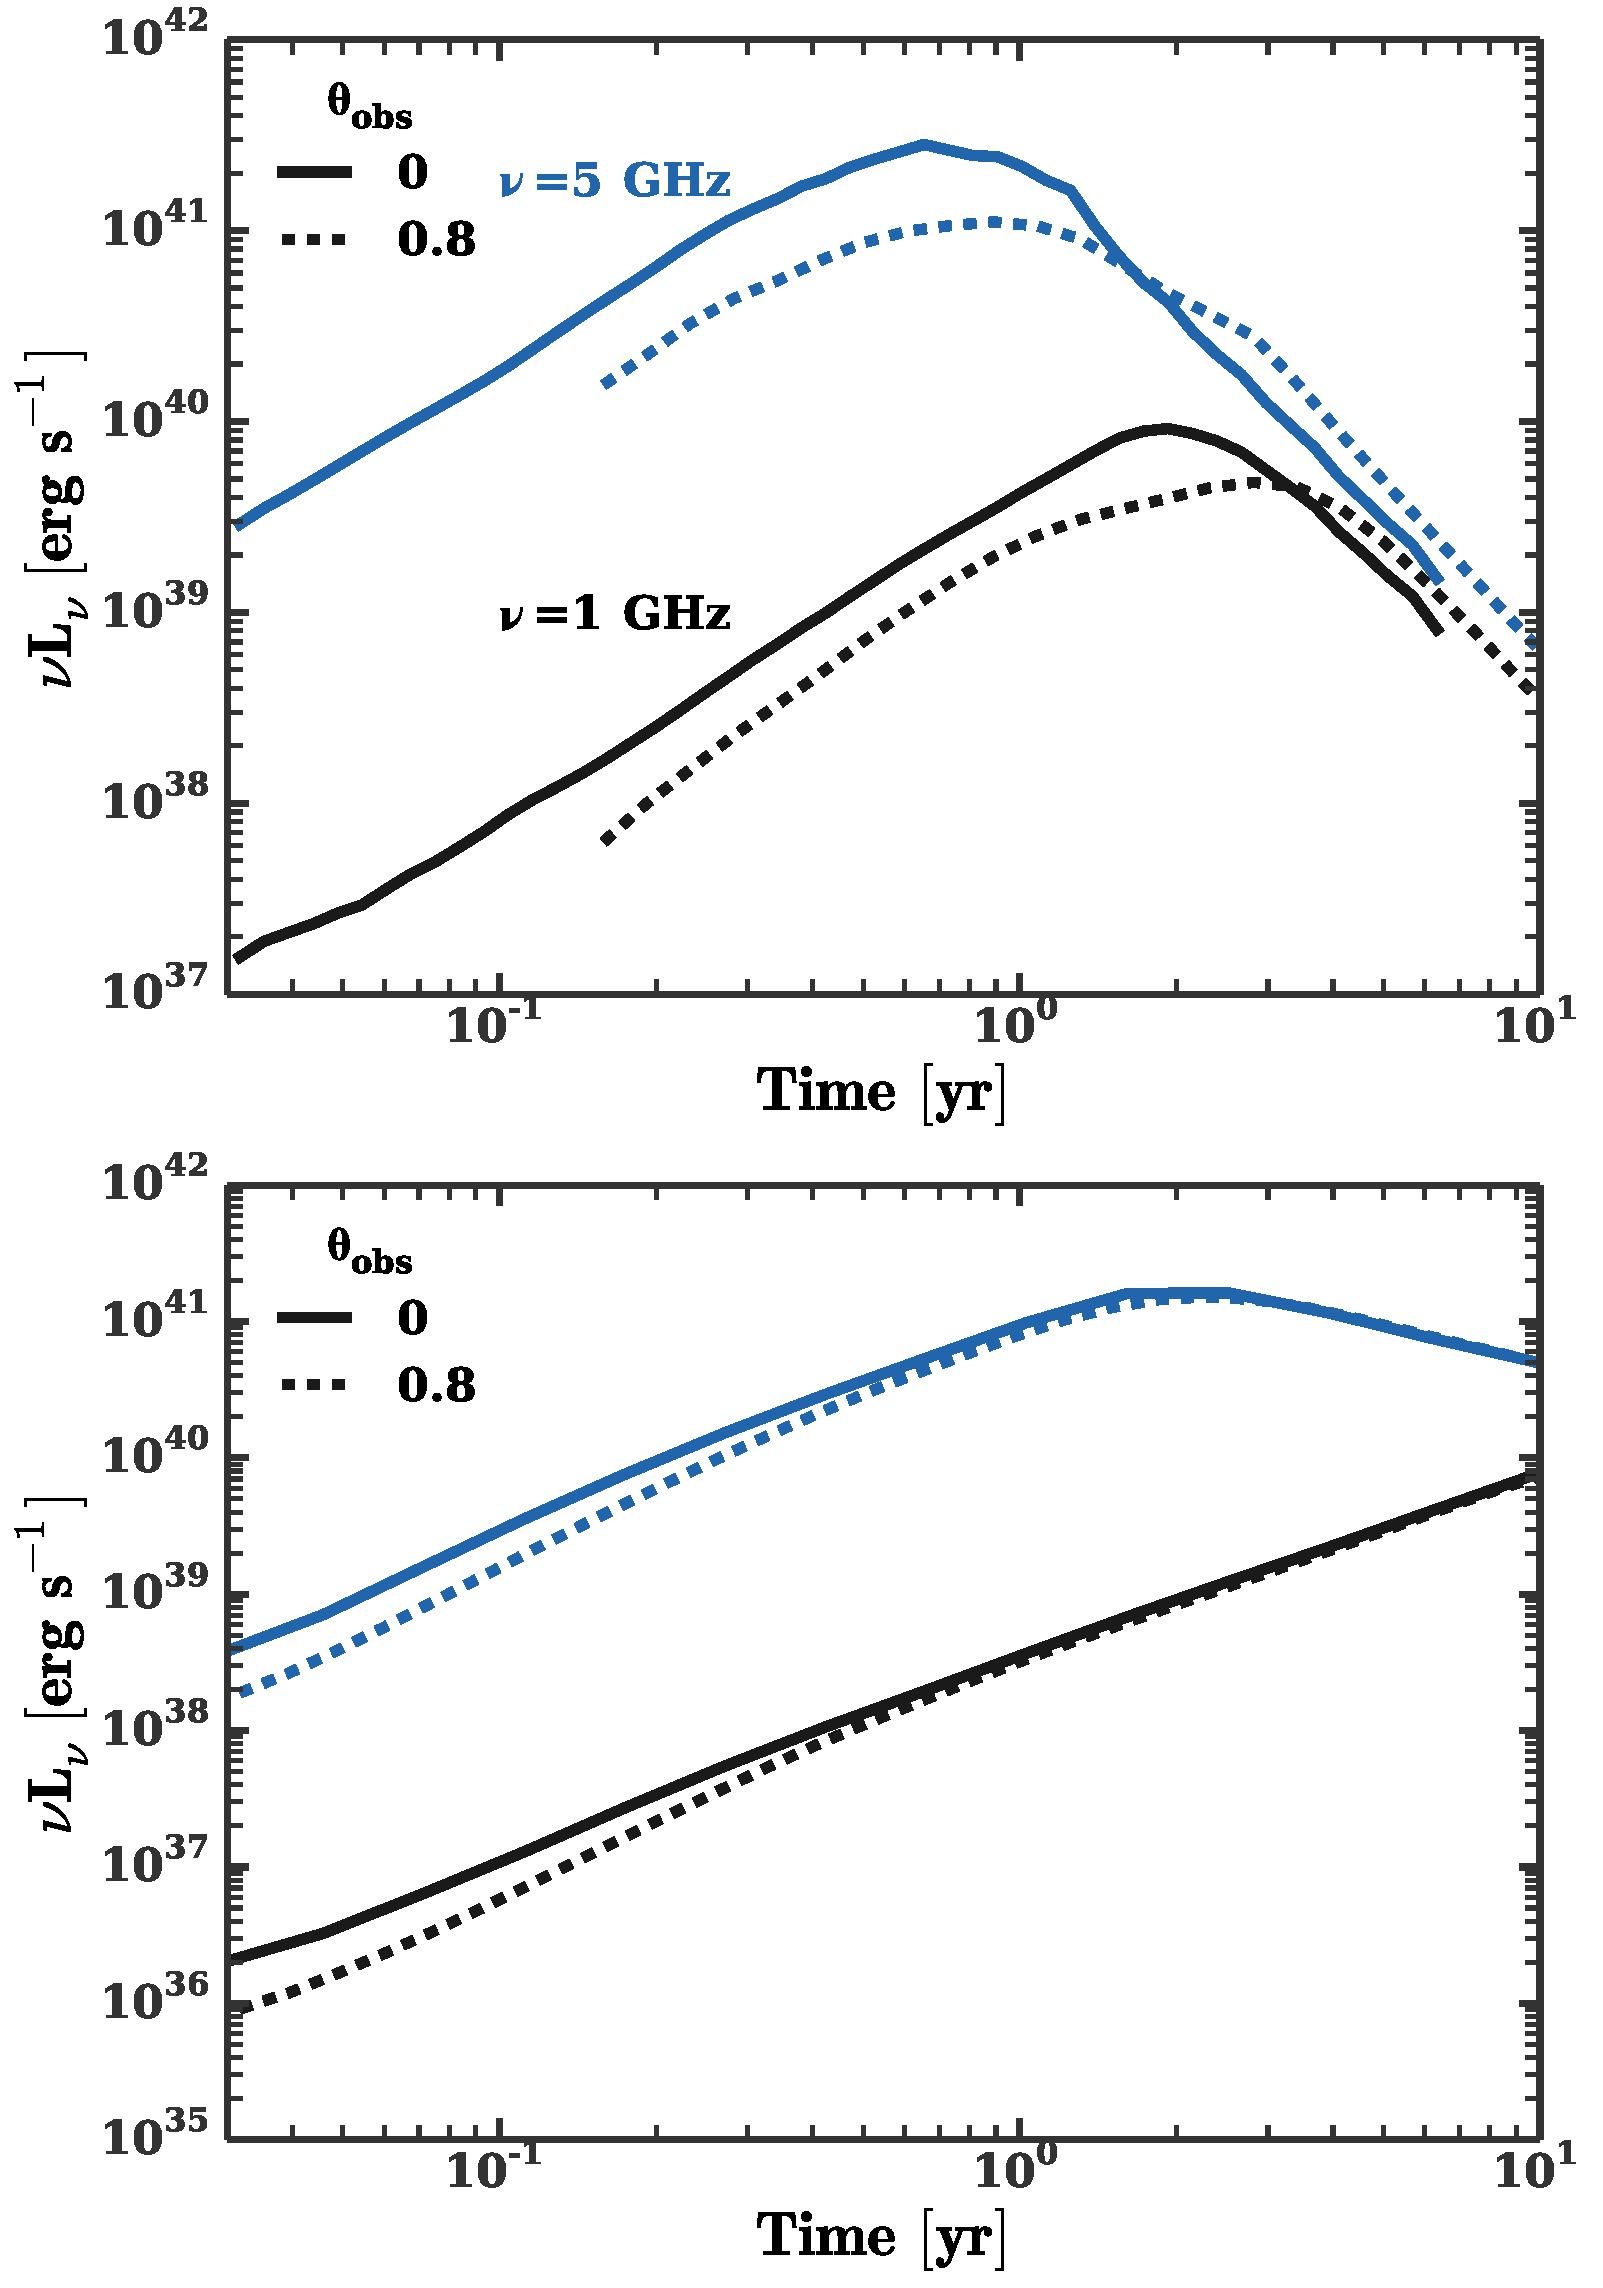
\includegraphics[width=8cm]{on_off.pdf}
\caption{\label{fig:onOff} Comparison of (2D) off- and on-axis light
  curves for $n_{18}=60$ cm$^{-3}$ (top) and $n_{18}=2000$ cm$^{-3}$
  (bottom) for frequencies of 1 and 5 GHz. The observer line of sight
  is taken to be at $\theta_{\rm obs}=0.8$ with respect to the jet
  axis. We assume an $n\propto r^{-1}$ density profile for
  $n_{18}=2000$ cm$^{-3}$, but take $n\propto r^{-1.5}$ for
  $n_{18}=60$ cm$^{-3}$ for computational convenience--this model was
  previously computed in \citet{Mimica+2015} and 1D results suggest
  that the density slope would have minimal impact on the results (see
  $\S$~\ref{sec:profileComp}).}
\end{figure}

\subsubsection{Effect of gas density profile}
\label{sec:profileComp}
Fig.~\ref{fig:cores} shows on-axis radio light curves for our fiducial
gas density profile, $n\propto r^{-1}$, and a core galaxy profile (equation~\ref{eq:cores}),
both with $n_{18}=2$ cm$^{-3}$.  The light curves differ by at most a
factor of a few. The core and cusp light curves are even closer at
higher densities, and virtually indistinguishable at $n_{18}=2000$
cm$^{-3}$. This is because for larger ambient densities, the jet only
samples small radii, where the core and cusp profiles are 
similar (see Fig.~\ref{fig:profiles}). It is only at lower densities,
for which the Sedov radius lies outside of the flattening of the core
density profile, that noticeable differences emerge. {\bf AG why are
  there differences at early times for $n_{18}=2$ cm$^{-3}$ but not
  $n_{18}=2000$ cm$^{-3}$. Is this simply an artifact of the starting
  radius?}

Fig.~\ref{fig:profs2} compares the 1D on-axis light curves for
density two density profiles: $n\propto r^{-1}$ and $n\propto r^{-1.5}$
with $n_{18}=60$. For most times the light curves are very close.
This is as expected, since the Sedov radius, $r_{\rm sedov}\sim
10^{18}$ cm. 

Overall we conclude that the radio light curve is insensitive to the
precise gas density profile, for a fixed value of the gas density near
the deceleration/Sedov radius.

\begin{figure} 
  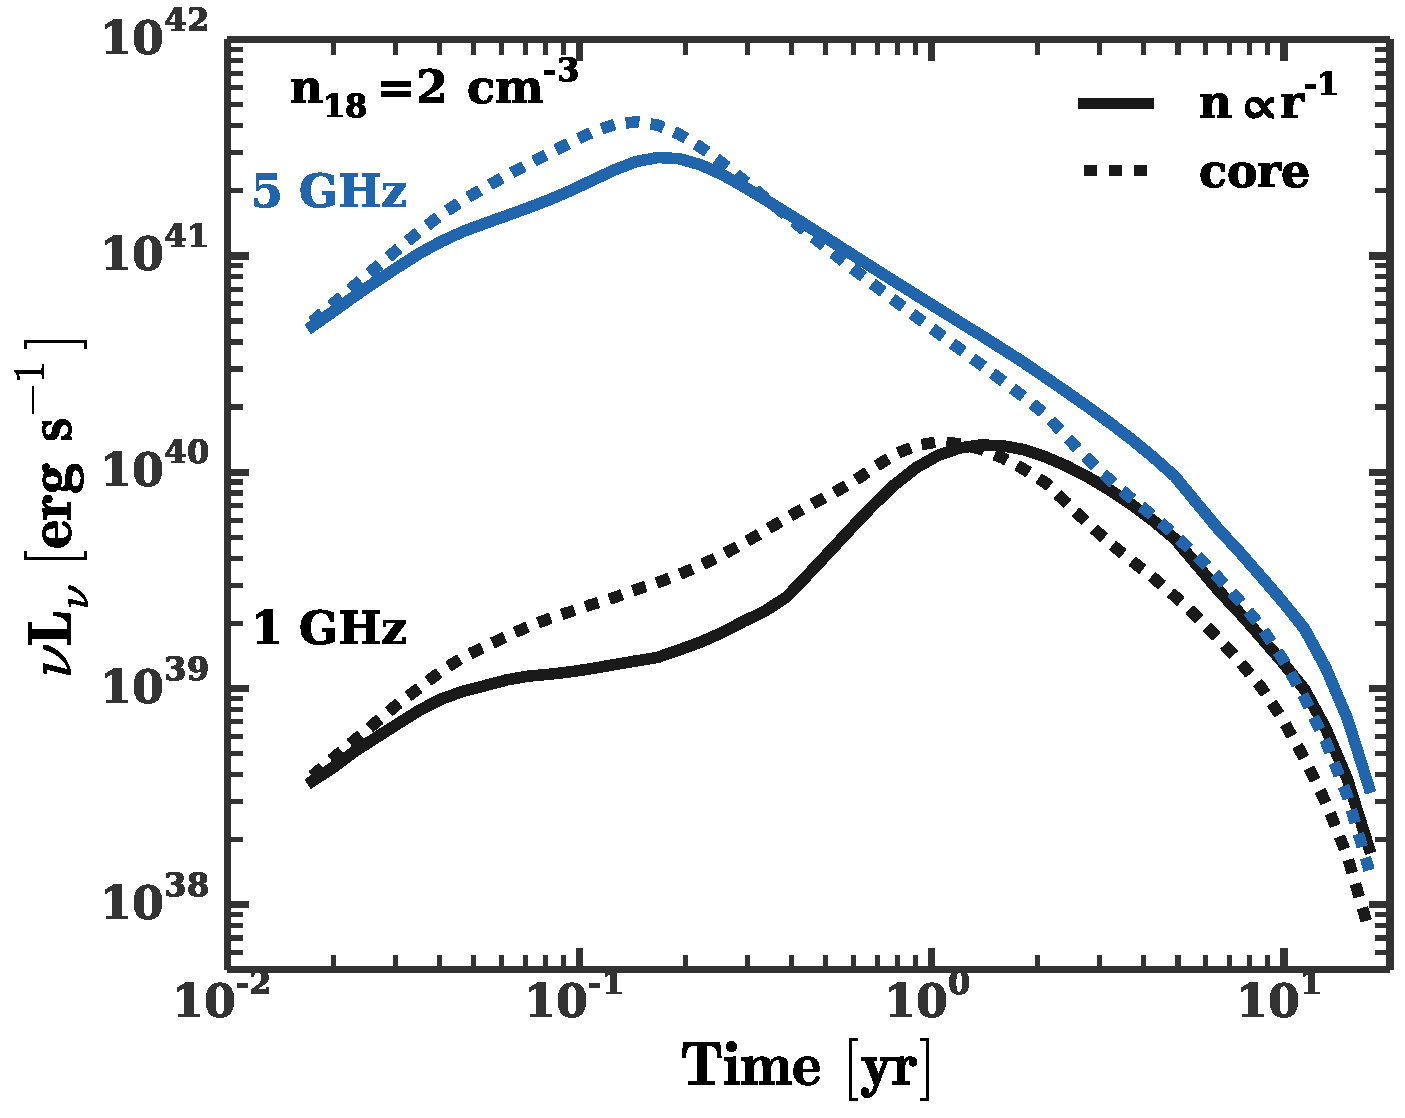
\includegraphics[width=8cm]{fig_cores.pdf}
  \caption{\label{fig:cores} Comparison of (on-axis) light curves for
    $n_{18}=2$ cm$^{-3}$ and two different CNM gas density profiles: $n\sim
    r^{-1}$ and the core galaxy profile from \eqref{eq:cores} with
    $r_s=10^{18}$ cm.}
\end{figure}


\begin{figure} 
  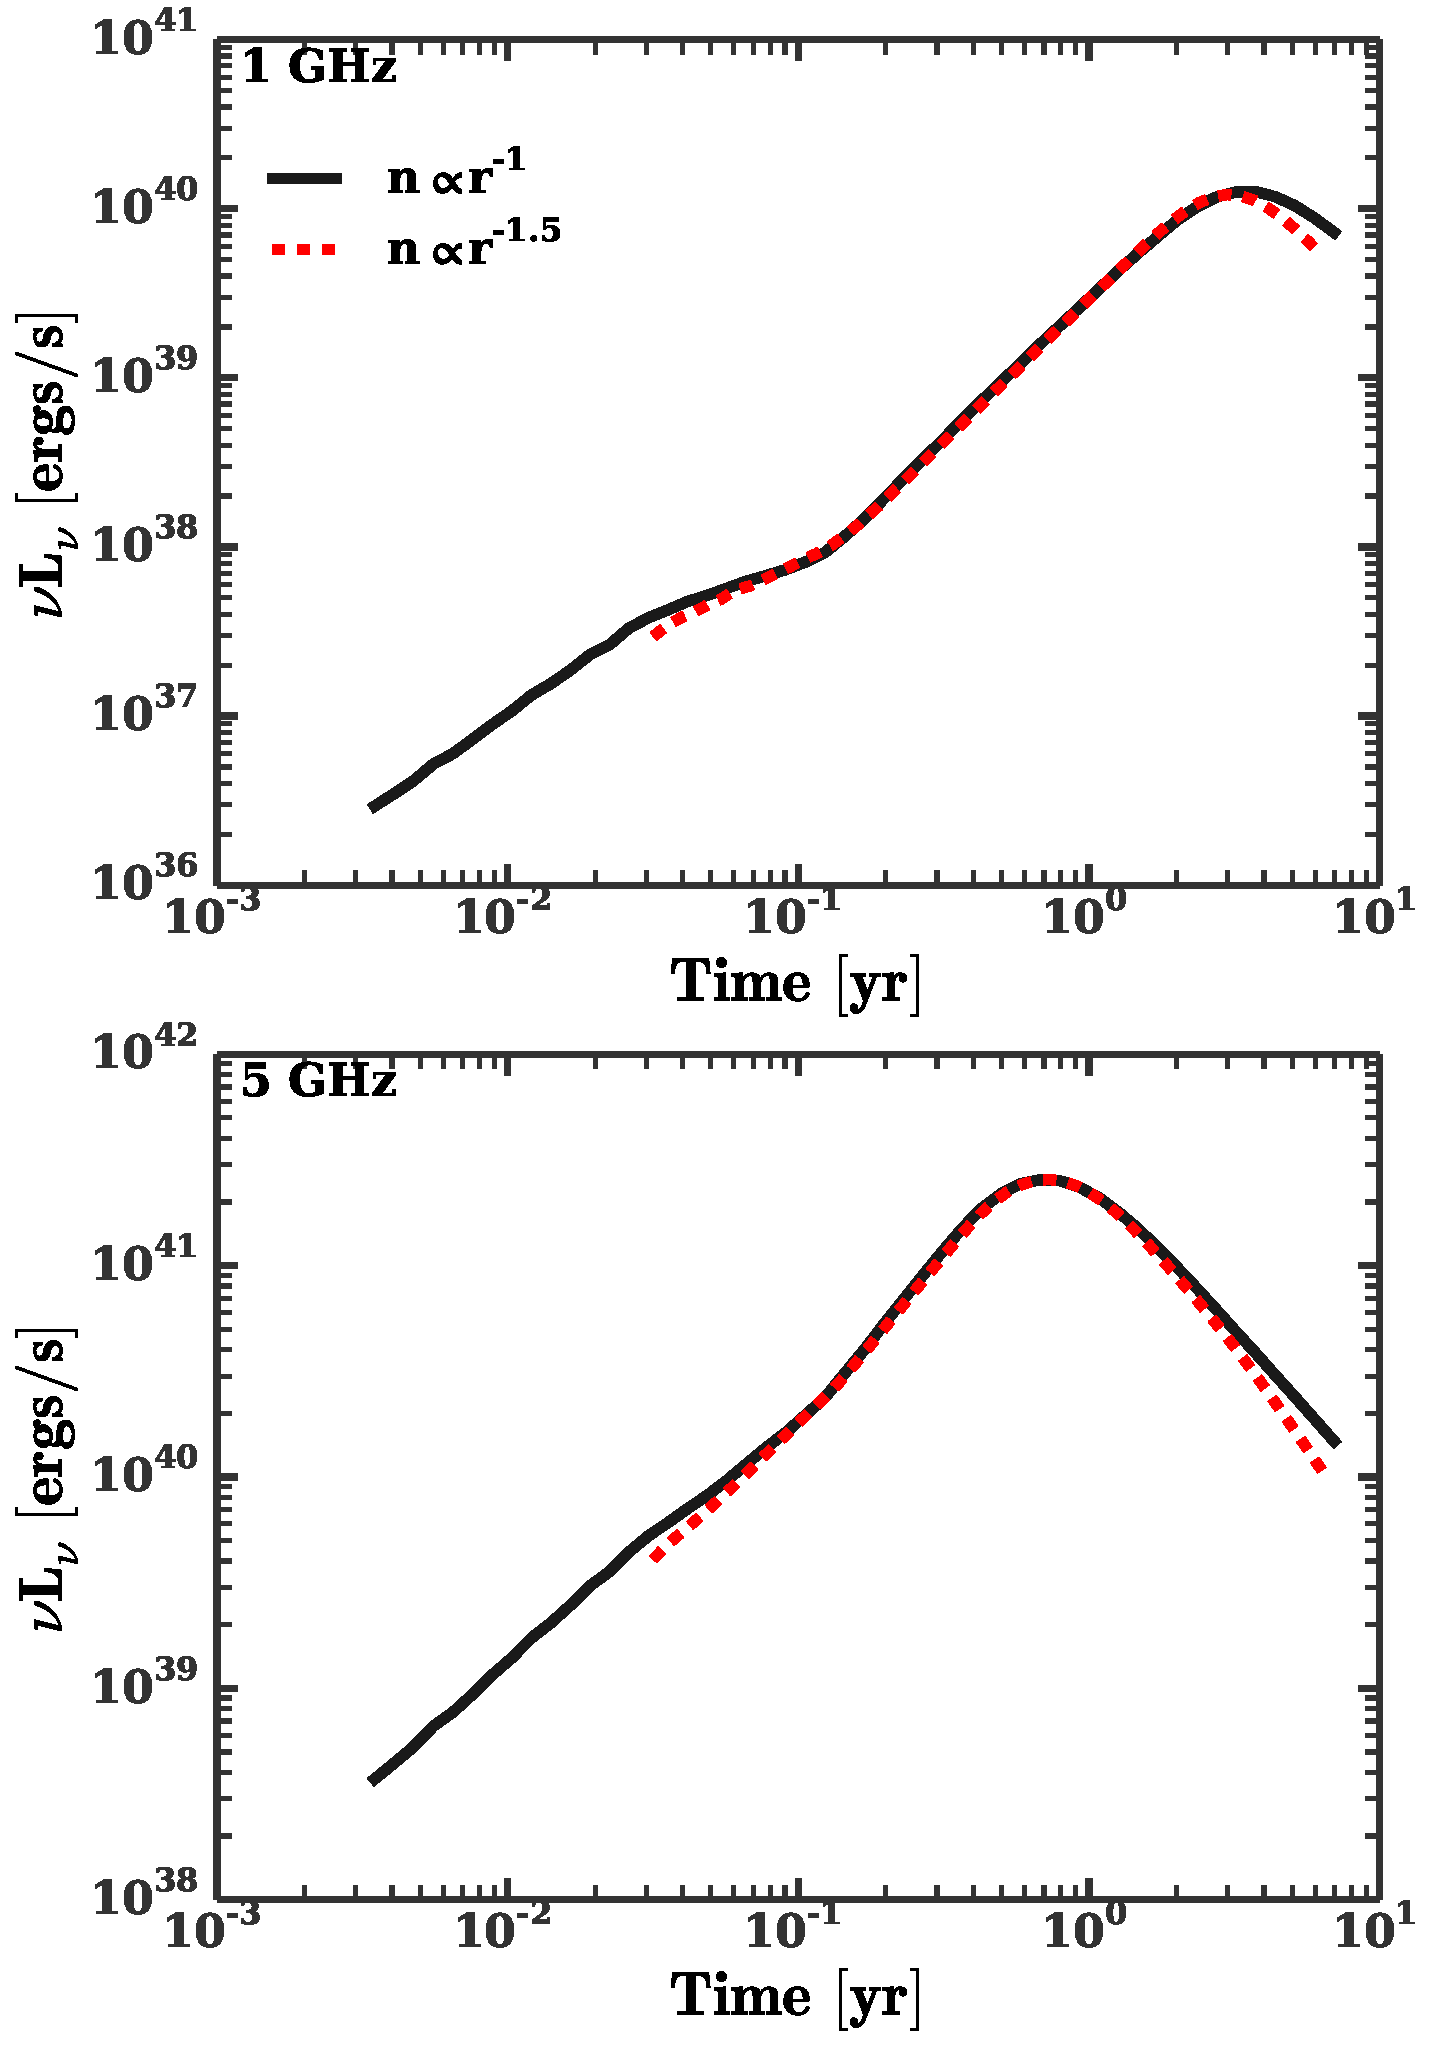
\includegraphics[width=8cm]{profs2.pdf}
  \caption{\label{fig:profs2} Comparison of (on-axis) light curves for
    $n_{18}=60$ and two different CNM gas density profiles: $n\propto
    r^{-1}$ ({\it solid black}) and $n\propto r^{-1.5}$ ({\it dashed
      red}).}
\end{figure}

\subsubsection{Contributions of the reverse shock}
Our calculations shown in Figs.~\ref{fig:1D2DB}$-$\ref{fig:cores}
include only emission from the forward shock (shocked CNM).  In
principal the reverse shock (shocked jet) may also contribute to the
radio light curve.
% However, as we describe in this section its contribution will be
% negligible, at least for high energy jets.

The fraction of the initial kinetic energy of the jet which is
dissipated by the reverse shock provides a first-order estimate of its
maximum contribution to the radio light curve.  Fig.~\ref{fig:diss}
shows the fraction of the slow component ($\Gamma=2$) kinetic energy
dissipated by the reverse shock as a function of isotropic jet
luminosity and CNM denisty $n_{18}$, as estimated by integrating the
shock evolution determined from the jump conditions (see
Appendix~\ref{sec:reverse} for details).  For this estimate, we
approximate the jet as a constant source of duration $t_0 = 5 \times
10^{5}$ s.  The parameters of our numerical solutions are shown as red
squares in Fig.~\ref{fig:diss}.
% {\bf AG
%careful shocks may be emitting at different frequencies. Also this
%energy is not necessarily lost...As we discussed upper bound
%interpretation may be naive}.

Fig.~\ref{fig:diss} shows that for high ambient densities and/or low
energy jets, the reverse shock dissipates an order unity fraction of
the kinetic energy of the jet.  However, this is somewhat deceptive
because for high energy jets the reverse shock emission will be
strongly attenuated by self absorption for observer frequencies below
10 GHz.  This is illustrated in Fig.~\ref{fig:reverse}, which shows
the 5 GHz light curve separated into contributions from the forward
and reverse shocks, respectively, calculated for $E = 5\times 10^{53}$
erg and $n_{18} = 2$.  Although the reverse shock contribution is
comparable to that of the forward shock at early times, it contributes
subdominantly to the total as compared to the forward shock due to
self-absorption near the front of the jet (which is not included in
the reverse shock light curve in Fig.~\ref{fig:reverse}).  While the
reverse shock dissipates an even larger fraction of the jet energy for
higher ambient density, its emission will be even more heavily
absorbed.  We conclude that reverse shock emission can be neglected
for the high energy jets with $E\gtrsim 10^{53}$ erg.

For low energy jets, we find that jet is crushed at early times, even
for low values of $n_{18}$, making the reverse shock structure more
challenging analyze in our simulations.  We defer a more detailed
study of the reverse shock in this case to future work.  {\bf BDM:
  Pere should add more here describing the issues with low energy
  jets}

As a final note, even if the reverse shock dissipates most of the
kinetic energy into thermal energy, this energy is still available to
be recoverted to kinetic energy through adiabatic expansion.  However,
the jet re-expansion will be relatively isotropic because the bulk
Lorentz factor of the shocked gas is now mildly relativistic.  The net
result will likely represent two Sedov-like `mushroom clouds' on
either side of the black hole (\citealt{Giannios&Metzger2011}).


\begin{figure}
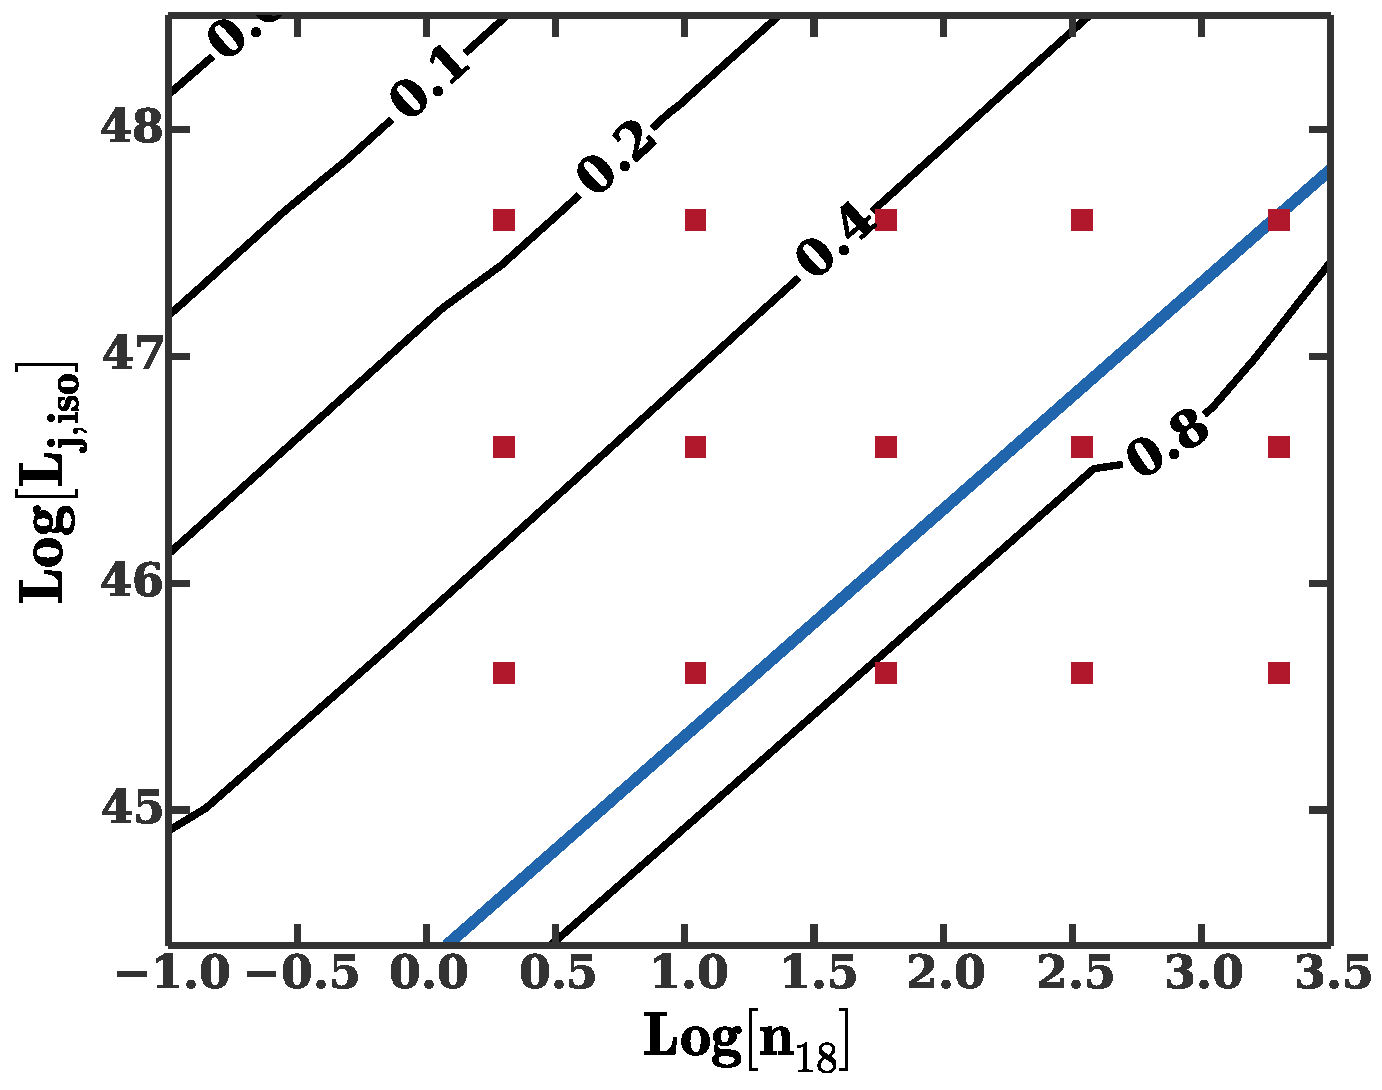
\includegraphics[width=8cm]{diss.pdf}
\caption{\label{fig:diss} Fraction of the slow component
  ($\Gamma=2$) kinetic energy dissipated by the reverse shock
  vs. the isotropic jet luminosity ($L_{\rm j,iso}$) and $n_{18}$.}
\end{figure}

\begin{figure}
  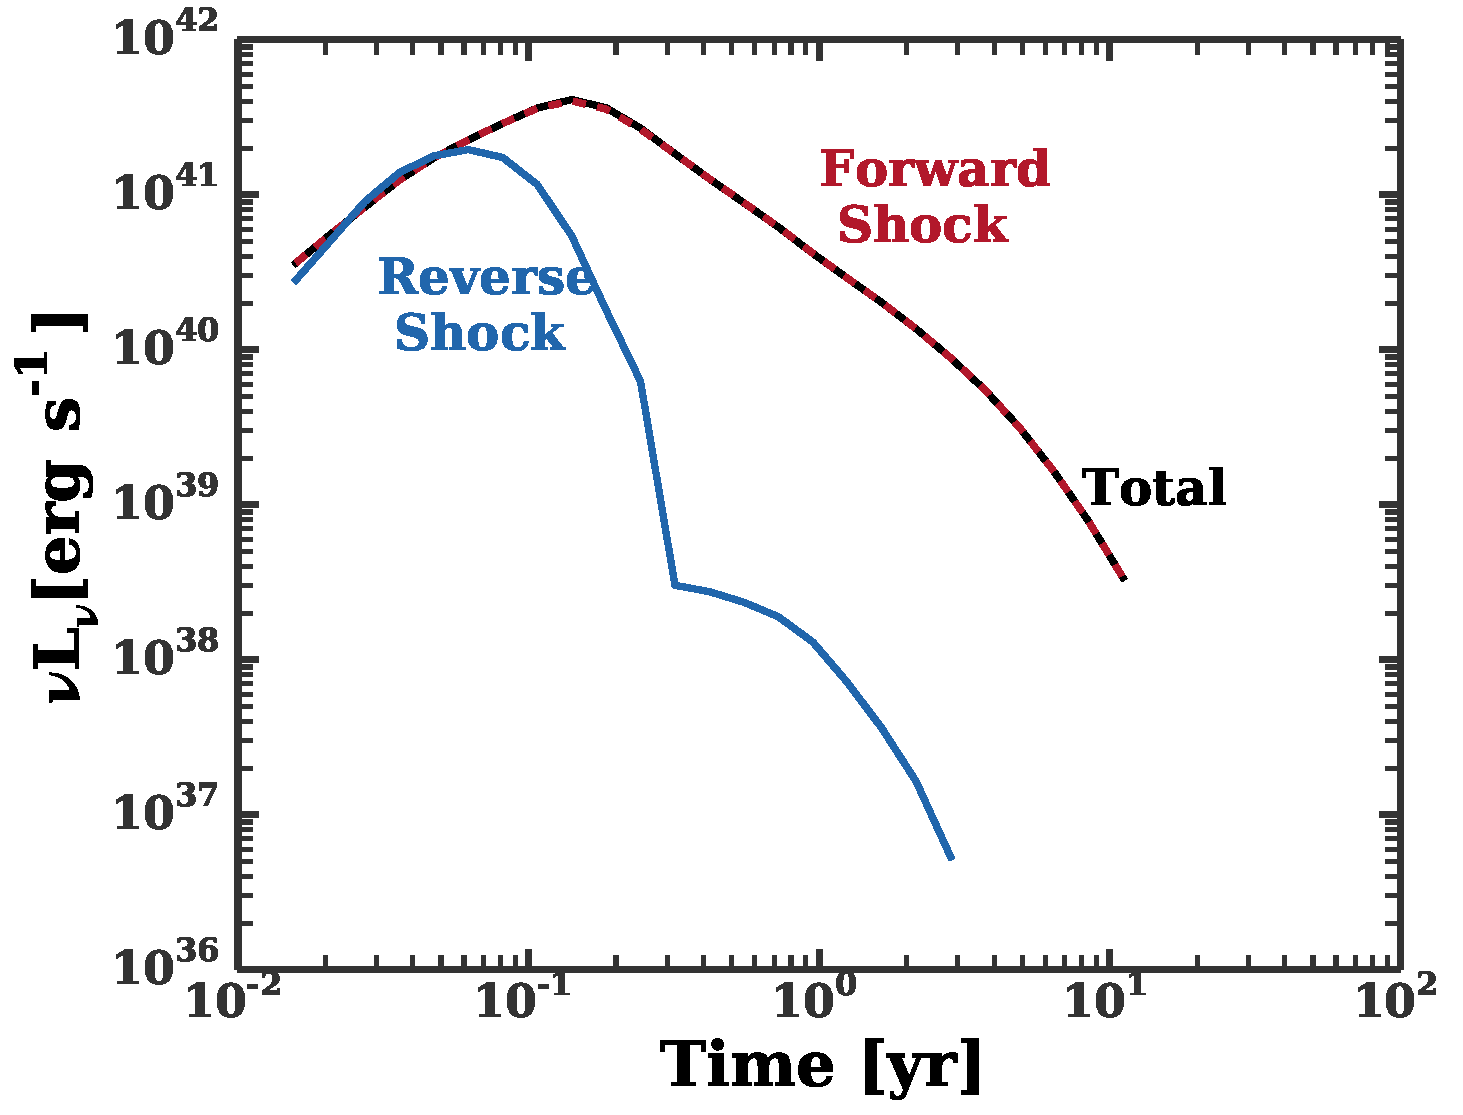
\includegraphics[width=8cm]{reverse.pdf}
  \caption{\label{fig:reverse} Reverse shock, forward shock, and total
    light curves for a $5\times 10^{53}$ erg jet propagating through
    our fiducial $n\propto r^{-1}$ medium with density normalization,
    $n_{18}=2$ cm$^{-3}$. The reverse shock emission is absorbed, so
    that effectively only the forward shock contributes to the total
    light curve.}
\end{figure}


\subsubsection{Overview of results}
As summarized in Table~\ref{tab:jetParams}, we calculate light curves
for a grid of on-axis jet simulations for five different values of
$n_{18}$ (2, 11, 60, 345, and 2000 cm$^{-3}$) and three different
values of the (beaming-corrected) jet energy $E$ ($5\times 10^{51}$,
$5\times 10^{52}$, $5\times 10^{53}$ erg). 

The left-hand side of Fig.~\ref{fig:jetContours} shows contours of the
peak luminosity for the slow component and total light curves across
this grid. In general, the slow component dominates for large
densities and small frequencies.  The peak luminosity of the slow
component falls off for low ambient gas densities, especially at 30
GHz. However, the fast component compensates for this decline, so that
the total peak luminosity is very weakly dependent on density across
the entire grid {\bf AG Not satisfying. Seems very coincidental and
  model dependent}.

\begin{figure}
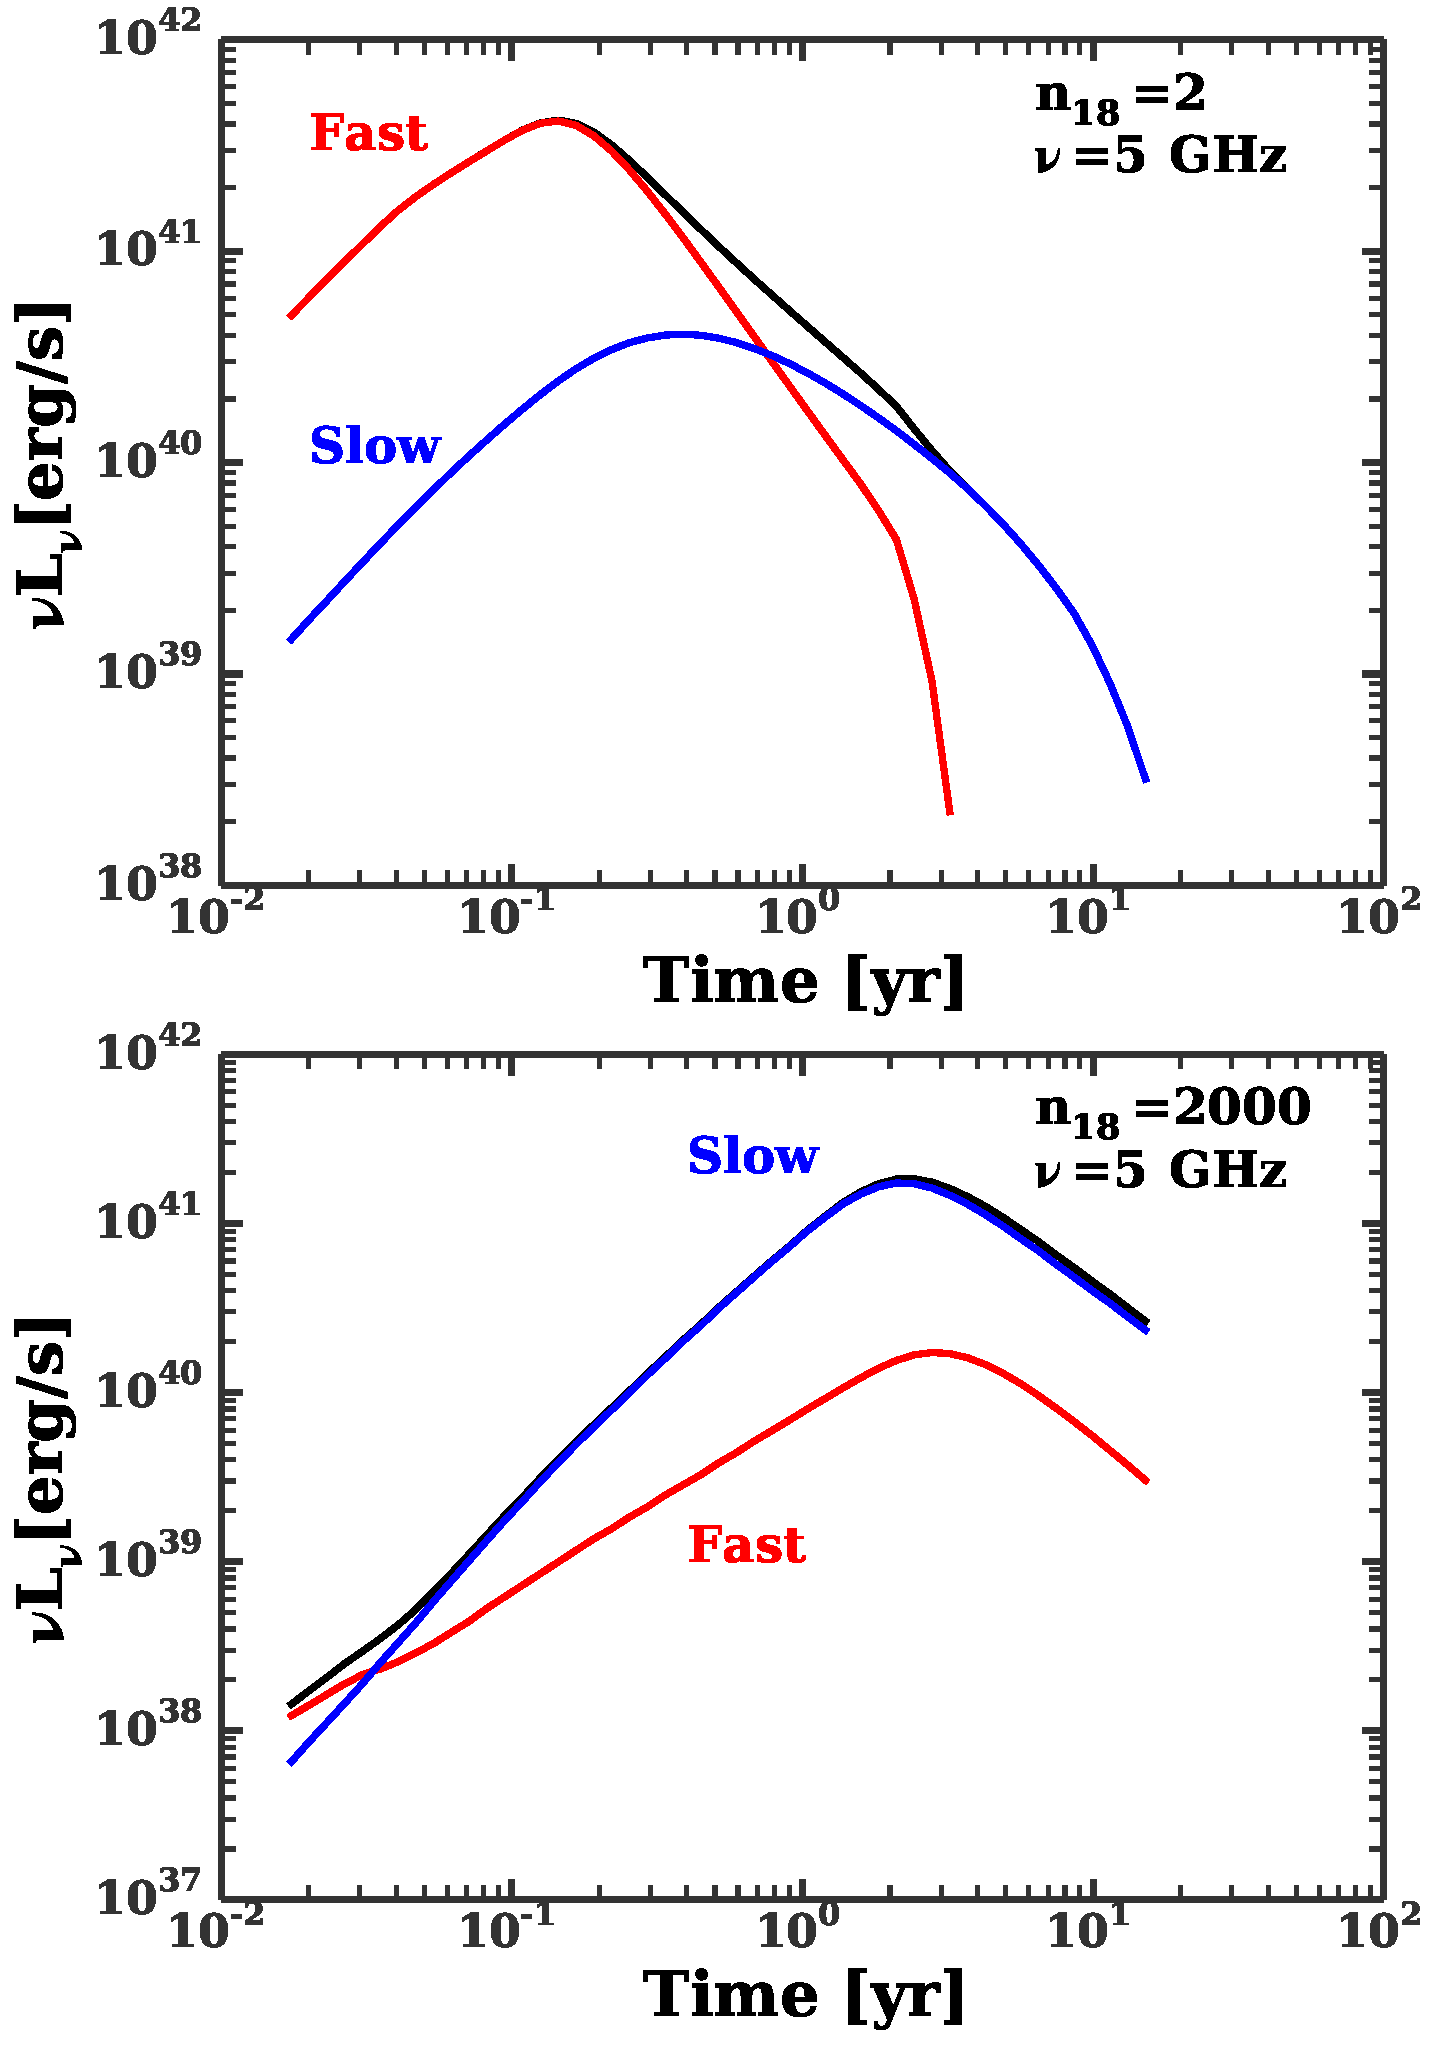
\includegraphics[width=8cm]{components.pdf}
\caption{\label{fig:components} Contributions from the fast
  (\textit{red}) and slow (\textit{blue}) to the 5 GHz light curves
  (\textit{black}) for $n_{18}=2$ cm$^{-3}$ (\textit{top}) and
  $n_{18}=2000$ cm$^{-3}$ (\textit{bottom}).}
\end{figure}


The right hand side of Fig.~\ref{fig:jetContours} shows comparisons of
the numerical results for the slow component with the results of
equation~\eqref{eq:peakLum}. For large $n_{18}$, the numerical results for
peak luminosity scale with density, jet energy, and frequency roughly
as expected for ``Case 2.'' For 30 GHz and low ambient gas densities,
the numerical results asymptotically approach the ``Case 1'' scalings.

The left-hand side of Fig.~\ref{fig:ContoursTp} shows contours of the
peak time for the slow component and total light curves. The
right-hand side of Fig.~\ref{fig:ContoursTp} shows the Case 2 peak
time from equation~\eqref{eq:peakTime} (with $t_2=49.9$ days), which
roughly reproduces the numerical results for high densities/low
frequencies. For lower densities, the numerical results diverge from
the analytic prediction, in part due to the contributions of the fast
component.  Furthermore, the peak time for the 30 GHz light curves
decreases with density for small $n_{18}$, as the emitting region is
optically thin at the deceleration time (``Case 1'').




\begin{figure*}
  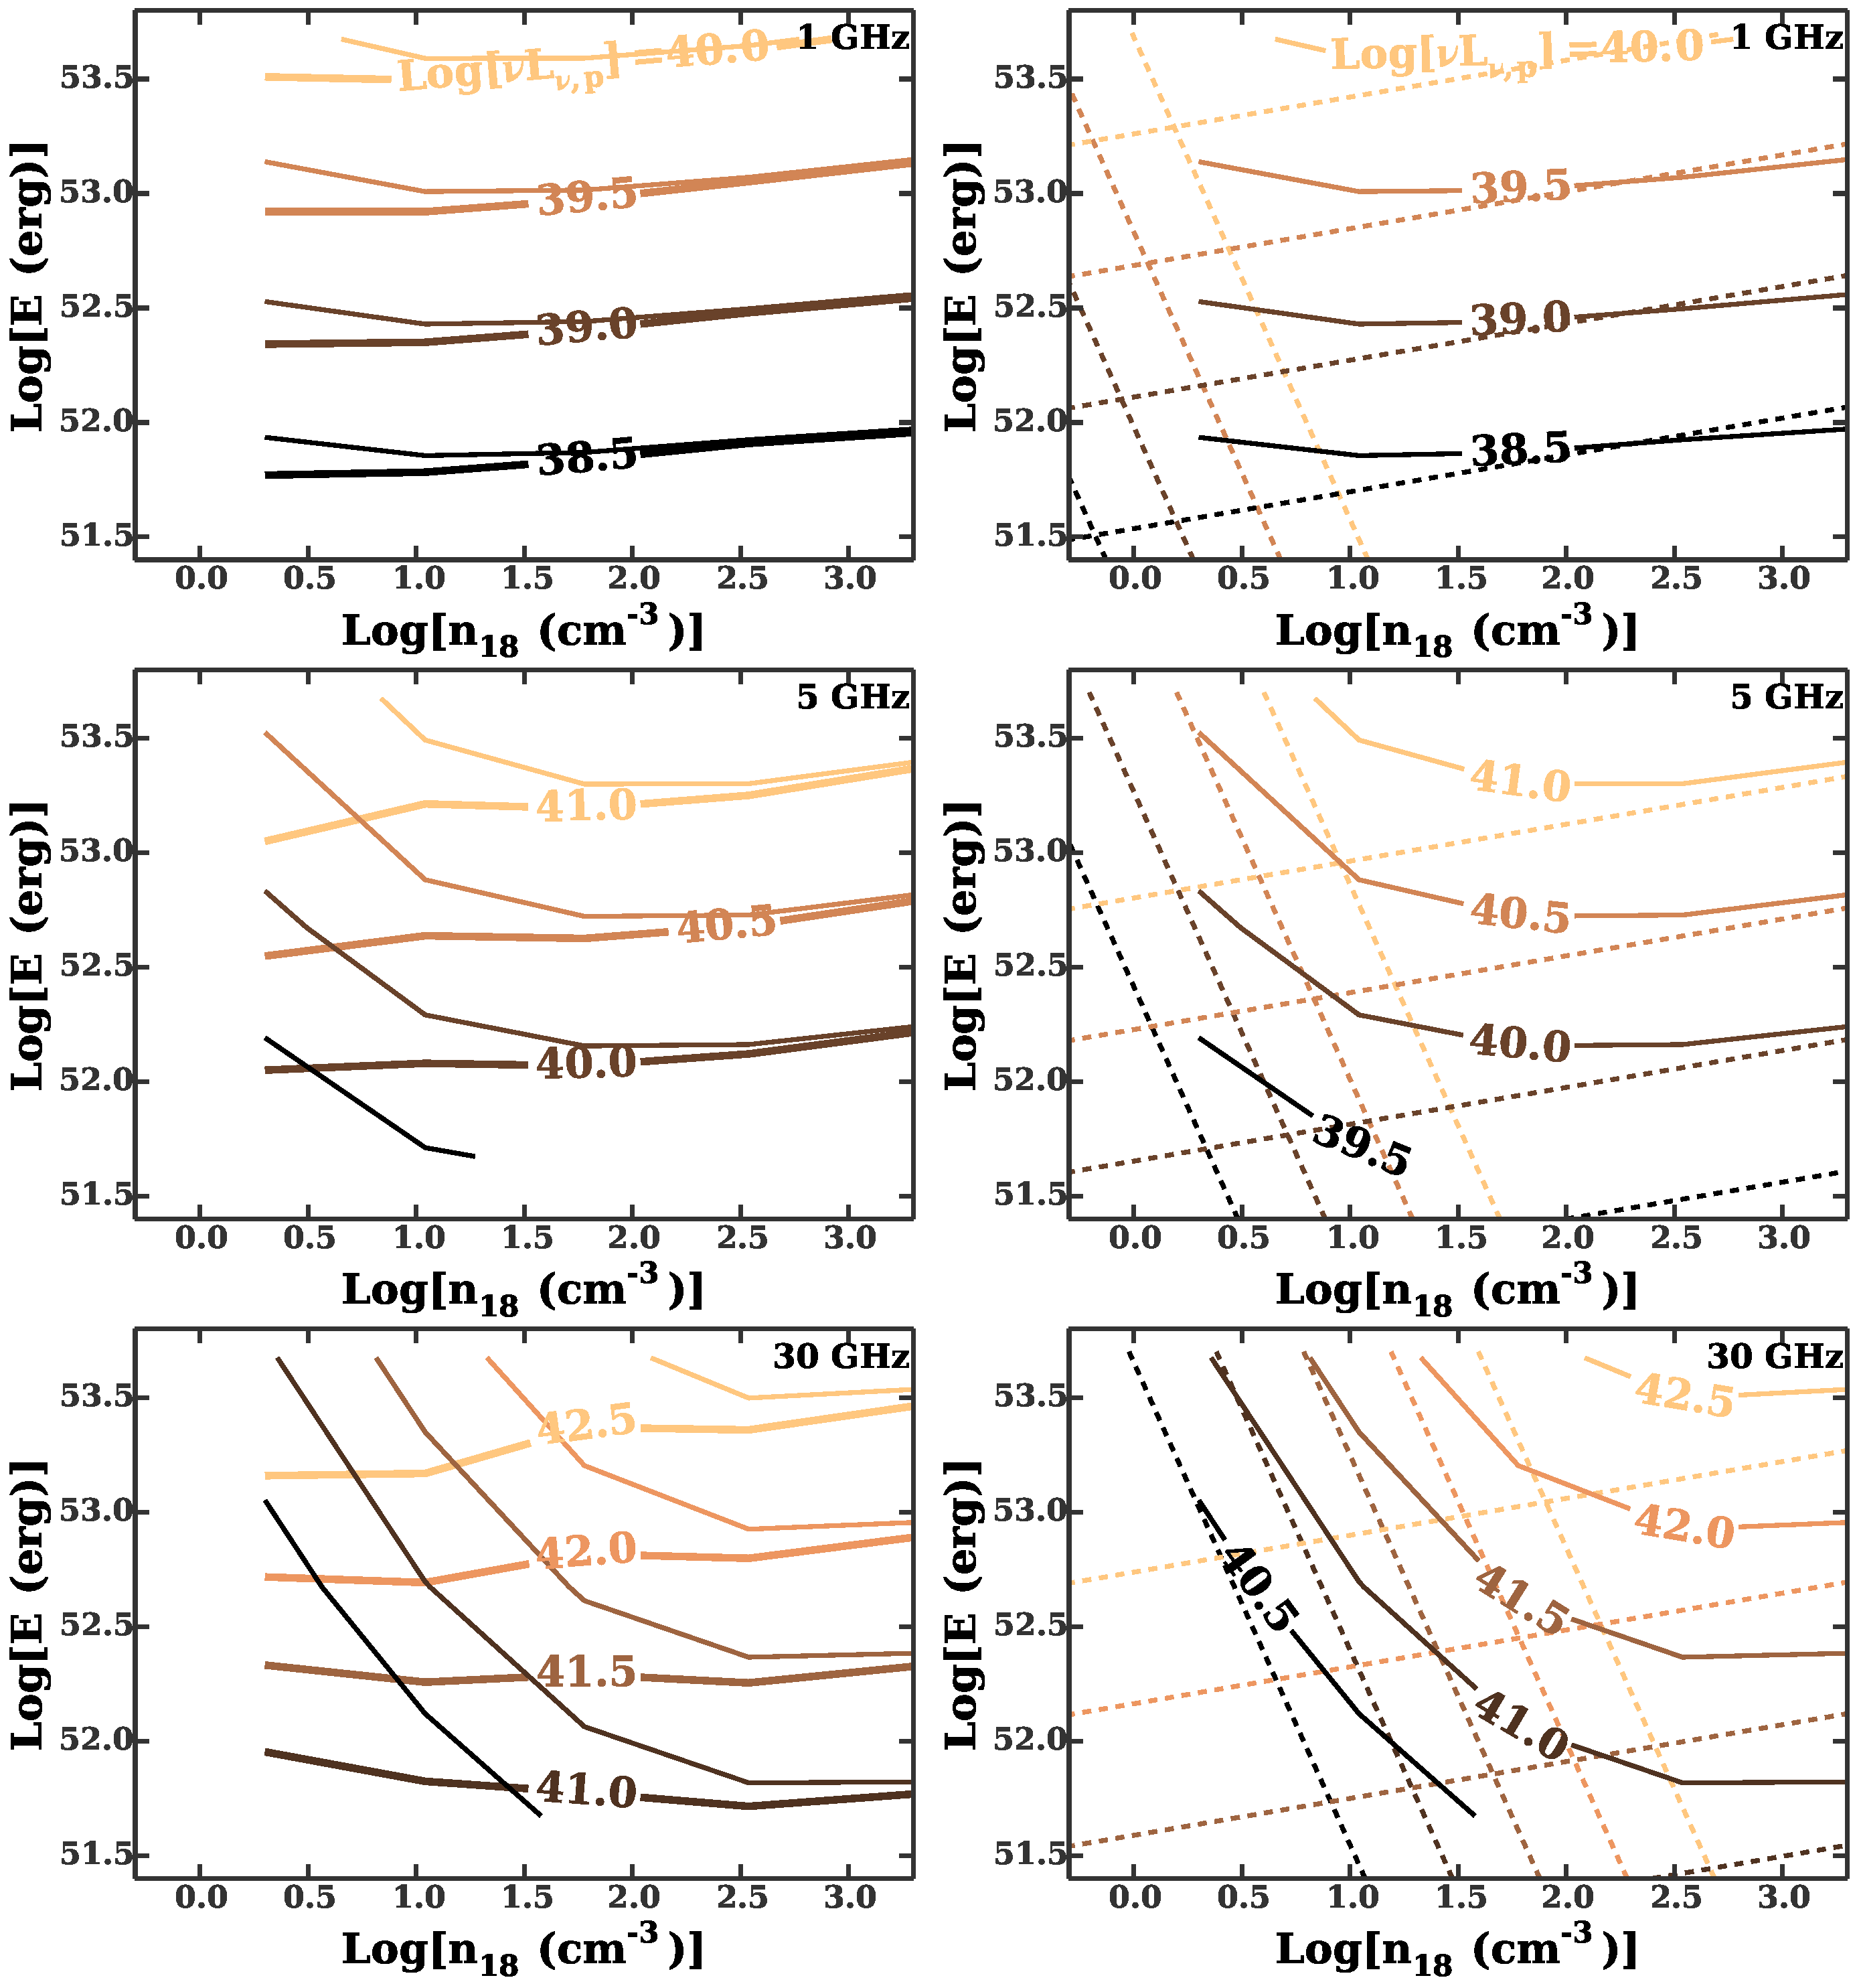
\includegraphics[width=16cm]{lp_contours_new.pdf}
  \caption{\label{fig:jetContours} {\it {Left:}} Thick lines show peak
    luminosity in the parameter space of jet energy and ambient gas
    density at $10^{18}$ cm, calculated from the grid of on-axis jet
    simulations in Table~\ref{tab:jetParams}. Thin lines show contours
    of peak luminosity for the slow component light curve
    (see $\S$~\ref{sec:numerical}). {\it Right:} Analytic scaling for the
    peak luminosity ({\it dashed}, see equation~\ref{eq:peakLum})
    compared to the numerical results for the slow component (solid
    lines).}
\end{figure*}

\begin{figure*}
  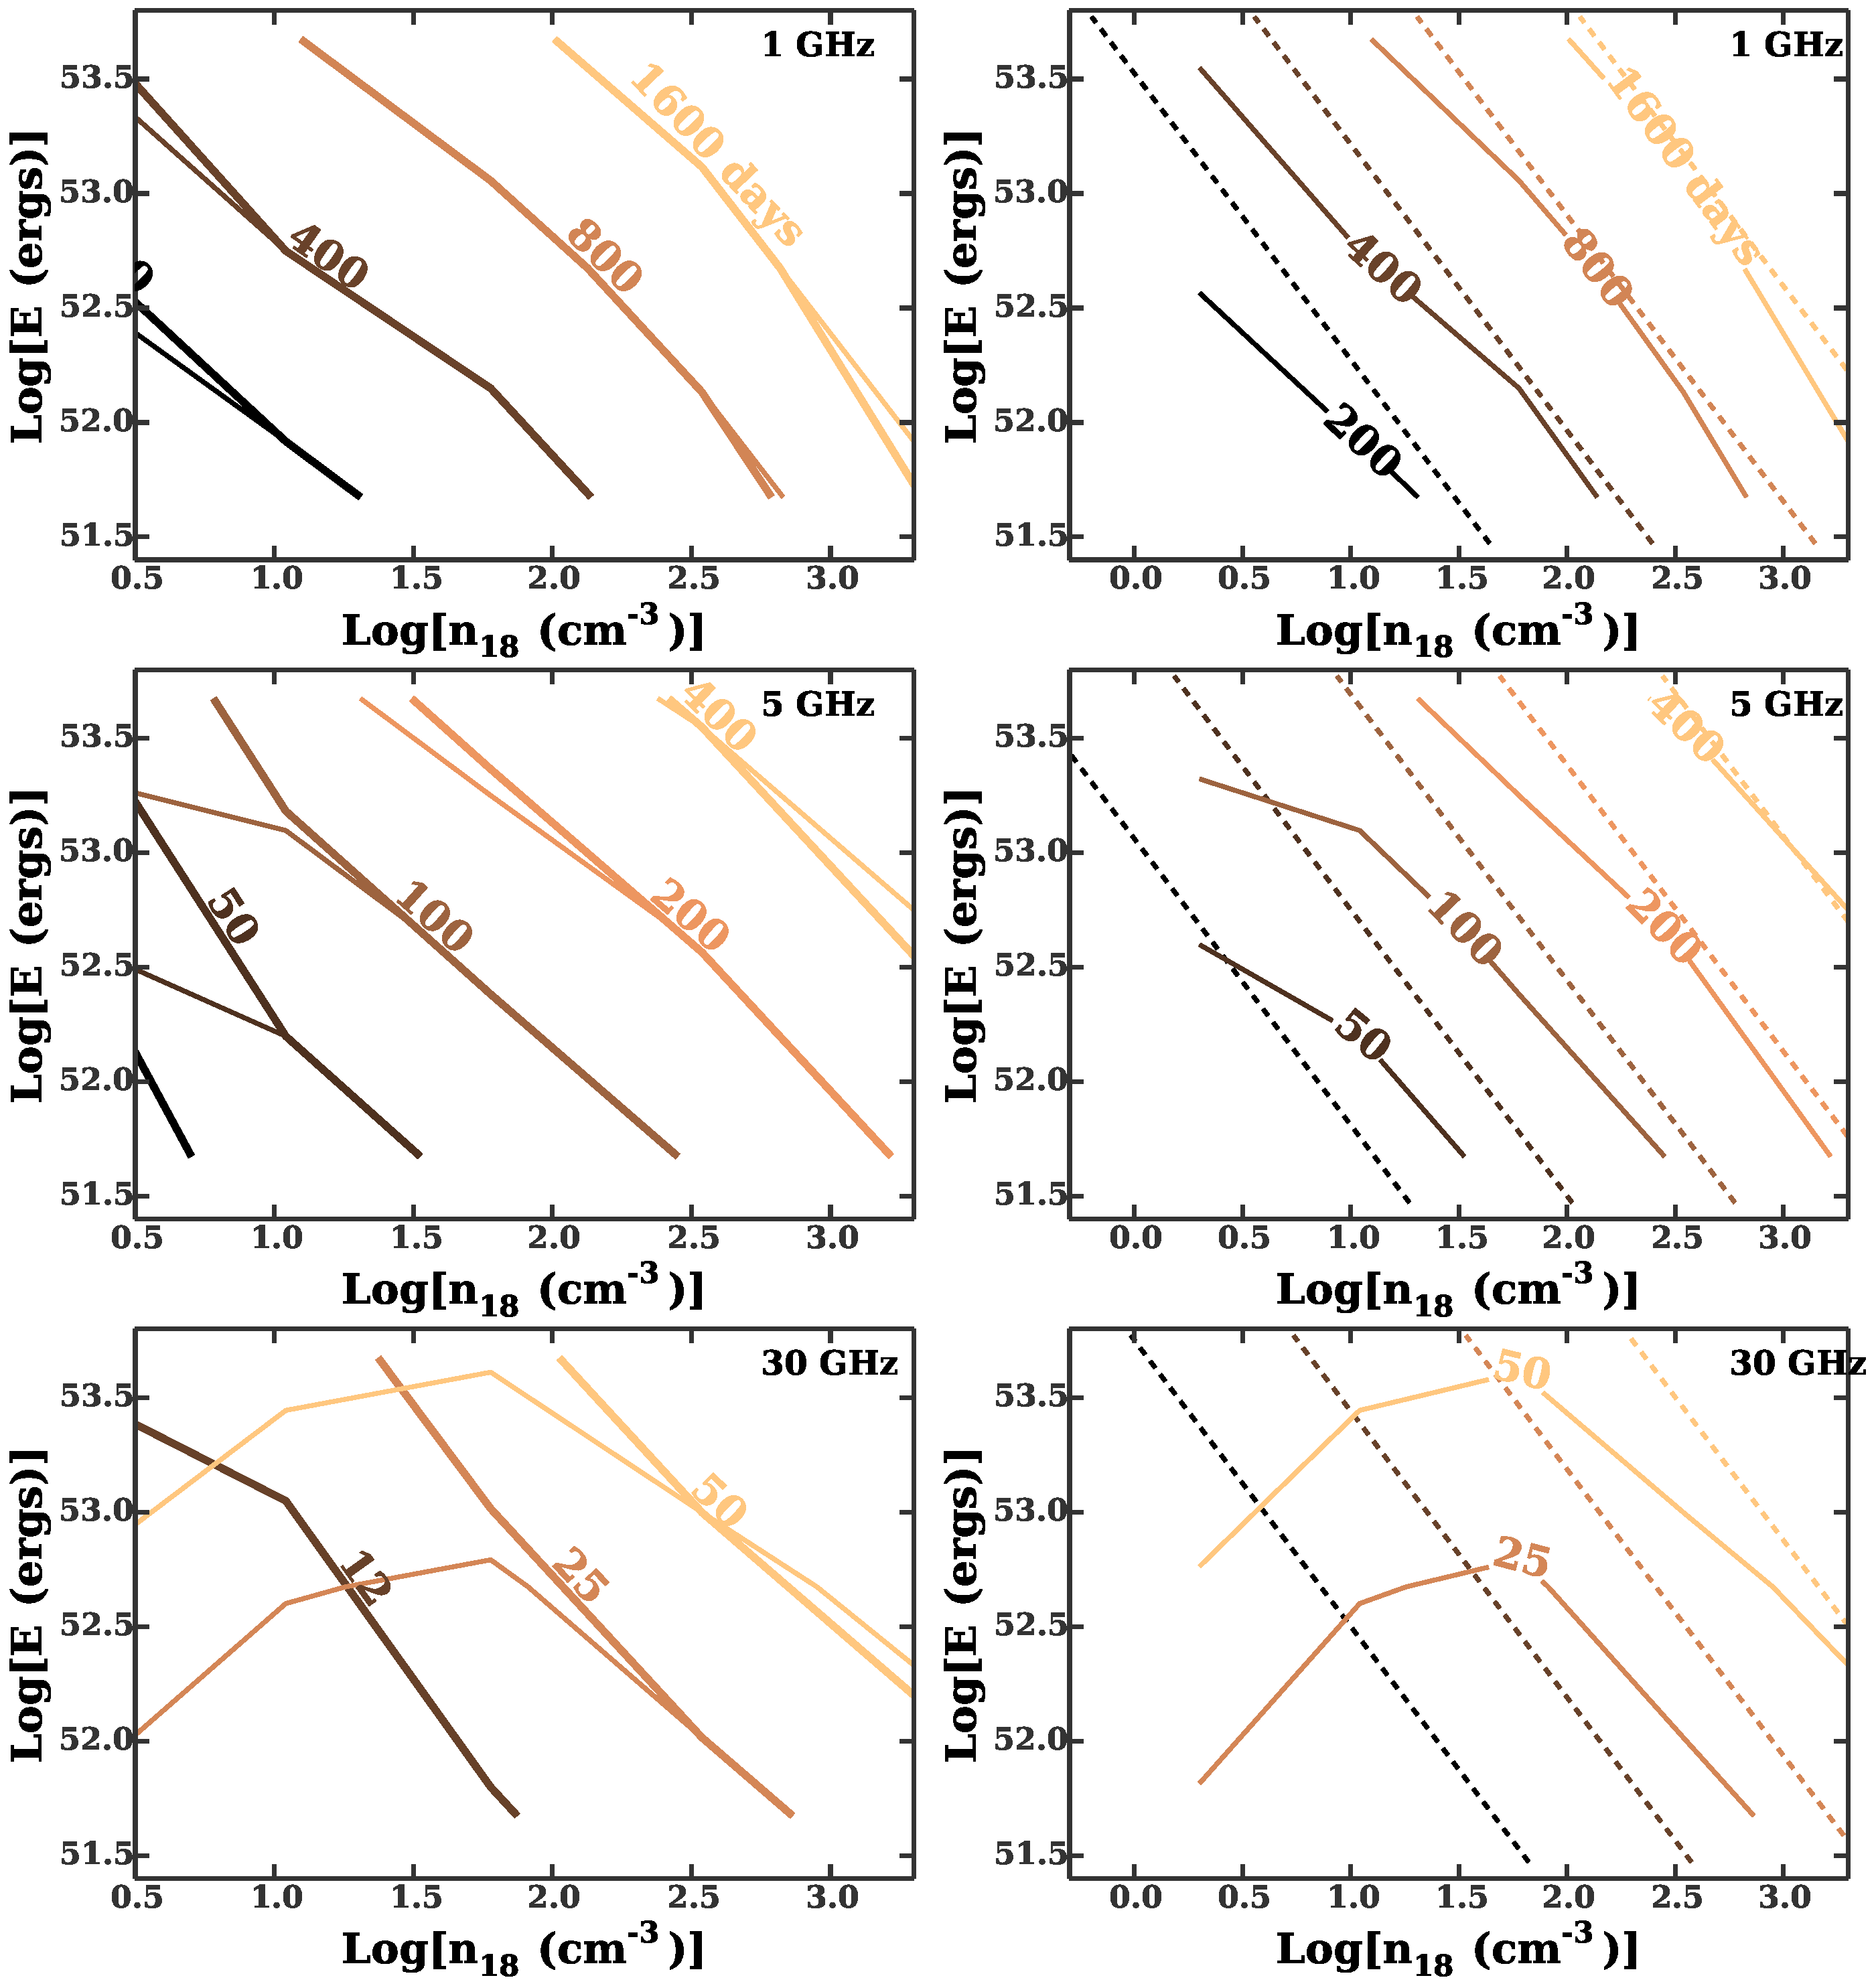
\includegraphics[width=16cm]{tp_contours_new.pdf}
  \caption{\label{fig:ContoursTp} {\it {Left:}} Thick lines show peak
    time in the parameter space of jet energy and ambient gas density
    at $10^{18}$ cm, calculated from the grid of on-axis jet
    simulations in Table~\ref{tab:jetParams}. Thin lines show contours
    of peak luminosity for the slow component light curve
    (see~\ref{sec:numerical}). {\it Right:} Analytic scaling for the
    peak luminosity ({\it dashed}, see equation~\ref{eq:peakTime})
    compared to the numerical results for the slow component (solid
    lines)}
\end{figure*}




\subsubsection{Comparison with radio detections and upper limits.}
The left panel of Fig.~\ref{fig:lightcurves} show radio upper limits
and detections for various TDE candidates (compiled from various
sources into Table 1 of \citealt{Mimica+2015}) together with on-axis
light curves for our fiducial $5\times 10^{53}$ erg jet (comparable to
SwJ1644) and three different ambient density normalizations: n$_{18}$:
2, 60, and 2000 cm$^{-3}$. All of the 5 GHz light curves fall above
the upper limits. However, we were unable to perform a 2D calculation
for $n_{18}=2$ cm$^{-3}$.  For $n_{18}=60$ cm$^{-3}$, the 2D light curve falls
$\sim$one order of magnitude below the 1D light curve after $\sim$ 10
years. Thus, we caution that the 1D light curves for $n_{18}=2$
cm$^{-3}$ likely overestimate the late time radio luminosity. For this
density even a SwJ1644 like jet would fall below existing upper
limits.

Multiple radio measurements from several months to a few years after a
tidal disruption flare would provide better constraints on the
presence of TDE jets. For example, suppose we have a TDE candidate
with a radio upper limit. Equation~\eqref{eq:peakLum}, provides a
constraint on the total energy of the jet

% luminosity distance $d_L$ away and the radio flux density at 5 GHz is
% constrained to be less than $S$. Then from equation~\eqref{eq:peakLum},
% we can constrain the energy of the jet to be

\begin{equation}
E\lsim 2 \times 10^{48} \left(\frac{S}{50 \,\mu{\rm Jy}}\right)^{1.1}
  \left(\frac{d_L}{200 \,{\rm Mpc}}\right)^{2.3} {\rm erg},
\end{equation}
%
where $S$ is upper limit for the flux density and $d_L$ is the
luminosity distance to the source, and we have set $n_{18}=1$. 

\section{Summary and Conclusions}
\label{sec:conc}

We calculate radio light curves for tidal disruption event jets
propagating through different circumnuclear (CNM) gas densities. We
simulate the jet propagation using both 1D and 2D hydrodynamic
simulations. We then post-process these to produce radio synchrotron
light curves. To isolate the effects of the density profile we take a
fixed two component jet model from \citet{Mimica+2015}, which produces
a good fit to the observed radio data in SwJ1644. We
consider a broad range of gas densities motivated by analytic
estimates of stellar wind mass injection and empirical constraints
based on observed distributions of Eddington ratios. Our conclusions
are summarized as follows.

\begin{enumerate}
\item We estimate the nuclear gas densities expected from injection of
  stellar wind material for different star formation histories. We
  find that that range of gas densities at 10$^{18}$ cm is $n_{18}
  \sim$ 0.5-2000 cm$^{-3}$.

\item The slope of the gas density profile depends on the slope of the
  stellar density profile. We expect a typical TDE host to have cuspy
  stellar density profile inside of a few pc, with $\rho_\star
  \propto r^{-1.7}$. This translates into a gas density profile $n
  \propto r^{-1}$. The radio light curve of a TDE jet is most
  sensitive to the density at the deceleration/Sedov radius (where it
  has swept up its mass in CNM gas). The light curve will be
  insensitive to changes in slope for fixed density at the
  deceleration radius.

\item We use the distribution of Eddington ratios (measured by
  \citealt{Kauffmann&Heckman2009} using $L[OIII]/\Mbh$) for a sample
  $\sim 10^{7} \Msun$ black holes from SDSS to obtain an empirical
  constraint on the average circumnuclear gas density, including all
  phases of gas. We find that $\sim90\%$ of galaxies in the sample
  have $n_{18}<10^{4} \, {\rm cm}^{-3}$, although we note that there is
  considerable uncertainty in translating an observed Eddington ratio
  to a circumnuclear gas density. TDE hosts would not fall on this
  high density tail, as TDE hosts have either weak or no detected OIII
  emission.

\item We take a jet model which fits the radio data for the SwJ1644
  transient (from \citealt{Mimica+2015}) and run it through a range of
  different density profiles. Motivated by the above results for the
  expected range of gas densities we take the density at $10^{18}$ cm,
  to be $n_{18}=2, 60,$ or 2000 cm$^{-3}$. We find bright radio
  emission at a few GHz across this entire range of densities, with
  the peak luminosity only weakly dependent on the chosen value of
  $n_{18}$.  For smaller densities the light curves peak earlier in
  time. Based on existing radio upper limits for tidal disruption
  event candidates, we show SwJ1644-like jet are absent in most TDEs
  as long as the density at $10^{18}$, $n_{18} \gsim  60$
  cm$^{-3}$. Prompt follow-up in the radio could provide tighter
  constraints on the existence of TDE jets.  
\end{enumerate}

\appendix
\section{Core Profile}
\label{app:core}
In $\S\ref{sec:profileComp}$ we compare the results of radio
light curves from jets propagating in core and cusp like gas density
profiles. See Fig.~\ref{fig:profiles} for a comparison of core and
cusp-like profiles. 

We use the following analytic expression to approximate the core
galaxy profile

\begin{align}
\begin{cases}
n=n(r_s) k(x) & 0.4 \leq x\leq 2.0\\
n = 2.0 n(r_s) (x/0.4)^{-0.95} & x < 0.4\\
n = 0.75 n(r_s) (x/2.0)^{-0.26} & x>2.\\
\end{cases}
\label{eq:cores}
\end{align}

Where, 

\begin{align}
  &x=r/r_s\\\nonumber
  &k(x)=\frac{45}{19} \frac{1}{x^{3/2}} \frac{1-x^{1.9}}{9-19
      x\frac{x^{0.9}-1}{x^{1.9}-1}}
\end{align}

To isolate the effects of the shape of the density profile, consider a
core density profile with $r_s=10^{18}$ cm, and $n_{18}=2000$
cm$^{-3}$: the same as our high density cusp model.

\section{Peak Luminosities and times}
\label{app:analyt}
\citet{Leventis+2012} present analytic scaling relations for the
synchrotron flux of a spherical blast wave propagating through a
medium with a power law density profile, $n\propto r^{-k}$.  Here we
make use of their results to estimate the peak radio flux of the slow
(sheath) component of the jet.

During the late-time, Newtonian stage of the jet evolution,
synchrotron self absorption is important for frequencies below
\begin{align}
  \nu_{\rm sa}=&C_1(p, k) E_{54}^{\frac{10 p-k p -6 k}{2 (4+p) (5-k)}} n_{18}^{\frac{30 - 5 p}{2 (4 + p) (5 - k)}}
  \epsilon_e^{\frac{2 (p-1)}{4+p}} \epsilon_b^{\frac{p+2}{2 (4+p)}}\nonumber\\
  &t^{\frac{10 - 8 k - 15 p + 4 k p}{(4 + p) (5 - k)}}, 
\label{eq:nuSa} 
\end{align}
%
where $E = 10^{54}E_{54}$ erg is the blast wave energy and $C_1(p, k)$ is a normalization factor.  Equation~\eqref{eq:nuSa} is valid only if self-absorption frequency is greater than the synchrotron peak frequency,
\begin{equation}
\nu_m=C_2(p, k) E_{54}^{\frac{10-k}{2 (5-k)}} n_{18}^{-\frac{5}{2
    (5-k)}}  \epsilon_e^2  \epsilon_b^{1/2}  t^{\frac{4 k-15}{5-k}}.
\end{equation}
%
% The observing frequencies considered here ($\geq 1$ GHz), are also
% greater than $\nu_m$. 
The light curve will peak at the deceleration time (eq.~\ref{eq:tdec}) if the self-absorption frequency is below the observing band then (``Case 1''). Otherwise, it will occur after the deceleration time, when the self-absorption frequency crosses through the observing band (``Case 2''). The peak time for these two cases is

\begin{align}
t_{\rm p} \approx
\begin{cases}
  \frac{t_{\rm dec}}{2 \Gamma^2} \approx \left(100 \,
    E_{54}\right)^{1/(3-k)} \Gamma^{(2k - 8)/(3-k)} 
  n_{18}^{-1/(3-k)} {\rm yr} & {\rm Case\, 1}\\\\
  C_1(p, k)^{-\frac{(5 - k) (4 + p)}{10 - 8 k - 15 p + 4 k
      p}}E_{54}^{-\frac{-k p-6 k+10 p}{2 (4 k p-8 k-15 p+10)}}\\
  \times n_{18}^{-\frac{30-5 p}{2 (4 k p-8 k-15 p+10)}} \nu_{\rm
    obs}^{\frac{(5-k) (p+4)}{4 k p-8 k-15 p+10}}\\
  \times  \epsilon_b^{-\frac{(5-k) (p+2)}{2 (4 k p-8 k-15 p+10)}} \epsilon_e^{-\frac{2 (5-k) (p-1)}{4 k p-8 k-15 p+10}} & {\rm
    Case\, 2},
\end{cases}
\label{eq:tpeakGen}
\end{align}
%
where $\Gamma$ is the initial jet Lorentz factor. 
%The additional
%factor of $1/2 \Gamma^2$ for Case 1 is a correction accounting for the
%fact that the observed light curve will be compressed in time due to
%light travel time effects.

The unabsorbed flux at the peak frequency is given by
\begin{align}
  F_{\nu_m} =  C_3(p, k) E_{54}^{\frac{8-3 k}{2 (5-k)}}
  n_{18}^{\frac{7}{2 (5-k)}} \epsilon_b^{1/2} t^{\frac{3-2 k}{5-k}}
\label{eq:Fnum}
\end{align}
%
Extrapolating to the observer frequency gives 
\begin{align}
  \nu_{\rm obs} F_{\rm p} (\nu_{\rm obs}) &= \nu_{\rm obs}   F_{\nu_m}
  \left(\frac{\nu_{\rm obs}}{\nu_m}\right)^{-(p-1)/2}.
  \label{eq:Fpeak1}
\end{align}
%
Combining equations~\eqref{eq:tpeakGen}, ~\eqref{eq:Fnum},
and~\eqref{eq:Fpeak1}, we find
\begin{align}
  \nu_{\rm obs} F_{\rm p} (\nu_{\rm obs}) \propto
  \begin{cases}
    E_{54}^{\frac{k (p+5)-12}{4 (k-3)}} n_{18}^{-\frac{3 (p+1)}{4
        (k-3)}} \nu_{\rm obs}^{\frac{3-p}{2}}
    \epsilon_b^{\frac{p+1}{4}} \epsilon_e^{p-1} & {\rm Case \,
      1}\\\\
    E_{54}^{\frac{k(-(p-2))-10 p+3}{4 k (p-2)-15 p+10}} \\ \times
    n_{18}^{\frac{11 (p-2)}{4 k (p-2)-15 p+10}} \nu_{\rm
      obs}^{\frac{14 k (p-2)-47 p+57}{4 k (p-2)-15 p+10}} \\ \times
    \epsilon_b^{\frac{k (-(p-2))+p-8}{4 k(p-2)-15 p+10}}
    \epsilon_e^{-\frac{11 (p-1)}{4 k (p-2)-15p+10}} & {\rm Case \, 2}
  \end{cases}
  \label{eq:peakLumGen}
\end{align}


\section{Reverse shock}
\label{sec:reverse}
Here we estimate the fraction of the kinetic energy of the jet that is
dissipated by the reverse shock, as opposed to the forward shock whose
contribution is the focus of this paper.  From continuity, the
comoving density of a relativistic jet is given by
(e.g.~\citealt{Beloborodov&Uhm2006})
 \begin{align}
   n_{\rm j} =  \frac{L_{\rm j, iso}}{4 \pi r^{2}\Gamma_{\rm
       j}^{2}c^{3}m_p(1 + r \dot{\Gamma}/c\Gamma^{3})}
   \approx  \frac{L_{\rm j, iso}}{4 \pi r^{2}\Gamma^{2}c^{3}m_p},
\end{align}
%
where $L_{\rm j, iso}$ is the isotropic equivalent luminosity.  The
second term in the denominator can be neglected if the jet Lorentz
factor changes slowly ($\dot{\Gamma}_{\rm j} \ll c\Gamma^{3}/r$), a
condition which is satisfied at radii $r < r_{\rm dec}$ if $\Gamma$
changes slowly on a timescale $\gtrsim t_{\rm 0}$, where $t_{\rm 0}$
is the jet duration.

The common Lorentz factor of the shocked CNM and the shocked jet can be estimated using the relativistic shock jump condition and pressure equality between the forward and reverse shocks.  In the ultra-relativistic limit this gives,
\begin{equation}
\Gamma_{\rm sh} \underset{\Gamma_{\rm sh} \gg 1}= \Gamma\left[1 + 2\Gamma f^{-1/2}\right]^{-1/2},
\end{equation}
where
\begin{equation}
  f\approx 40\,  L_{\rm j,48} n_{18}^{-1} \Gamma_{10}^{-2} \, \left(\frac{r}{10^{18} {\rm
        cm}}\right)^{-1} 
\end{equation}
is the ratio of the density of the jet to that of the CNM.  This expression is inaccurate for mildly relativistic or non-relativistic, in which case we apply the more general expression for $\Gamma_{\rm sh}$ given by 
\citet{Beloborodov&Uhm2006} (their Fig.~6)
\begin{equation}
\frac{\Gamma^2-1}{\Gamma_{43}^2-1} f^{-1}=1 ,
\end{equation}
where
\begin{equation}
\Gamma_{43}=\Gamma \Gamma_{\rm sh} \left(1-\beta_{\rm sh} \beta_j\right),
\label{eq:gammaShGen}
\end{equation}
is the Lorentz of shocked jet in the frame of the unshocked jet. In the lab frame the reverse shock moves with a velocity
\begin{equation}
\beta_{\rm rs}=\frac{\beta_{\rm sh}(f)-\beta_{43}(f)/3}{1-\beta_{\rm
    sh}(f) \beta_{43}(f)/3}.
\label{eq:betars}
\end{equation} 
%
Equations~\eqref{eq:gammaShGen} and ~\eqref{eq:betars} can be used to
determine the radius of the shocks when the reverse shock crosses the
trailing edge of the jet and the value of $\Gamma_{\rm sh}$ at this
time.  The latter allows us to calculate what fraction of the initial
kinetic energy of the jet is dissipated at the reverse shock, instead
of being transferred to the shocked external medium via the forward
shock.



\clearpage
  \footnotesize{
    \bibliographystyle{mnras}
    \bibliography{master}
  }

\end{document}
